% Options for packages loaded elsewhere
\PassOptionsToPackage{unicode}{hyperref}
\PassOptionsToPackage{hyphens}{url}
%
\documentclass[
]{article}
\usepackage{amsmath,amssymb}
\usepackage{iftex}
\ifPDFTeX
  \usepackage[T1]{fontenc}
  \usepackage[utf8]{inputenc}
  \usepackage{textcomp} % provide euro and other symbols
\else % if luatex or xetex
  \usepackage{unicode-math} % this also loads fontspec
  \defaultfontfeatures{Scale=MatchLowercase}
  \defaultfontfeatures[\rmfamily]{Ligatures=TeX,Scale=1}
\fi
\usepackage{lmodern}
\ifPDFTeX\else
  % xetex/luatex font selection
\fi
% Use upquote if available, for straight quotes in verbatim environments
\IfFileExists{upquote.sty}{\usepackage{upquote}}{}
\IfFileExists{microtype.sty}{% use microtype if available
  \usepackage[]{microtype}
  \UseMicrotypeSet[protrusion]{basicmath} % disable protrusion for tt fonts
}{}
\makeatletter
\@ifundefined{KOMAClassName}{% if non-KOMA class
  \IfFileExists{parskip.sty}{%
    \usepackage{parskip}
  }{% else
    \setlength{\parindent}{0pt}
    \setlength{\parskip}{6pt plus 2pt minus 1pt}}
}{% if KOMA class
  \KOMAoptions{parskip=half}}
\makeatother
\usepackage{xcolor}
\usepackage[margin=1in]{geometry}
\usepackage{color}
\usepackage{fancyvrb}
\newcommand{\VerbBar}{|}
\newcommand{\VERB}{\Verb[commandchars=\\\{\}]}
\DefineVerbatimEnvironment{Highlighting}{Verbatim}{commandchars=\\\{\}}
% Add ',fontsize=\small' for more characters per line
\usepackage{framed}
\definecolor{shadecolor}{RGB}{248,248,248}
\newenvironment{Shaded}{\begin{snugshade}}{\end{snugshade}}
\newcommand{\AlertTok}[1]{\textcolor[rgb]{0.94,0.16,0.16}{#1}}
\newcommand{\AnnotationTok}[1]{\textcolor[rgb]{0.56,0.35,0.01}{\textbf{\textit{#1}}}}
\newcommand{\AttributeTok}[1]{\textcolor[rgb]{0.13,0.29,0.53}{#1}}
\newcommand{\BaseNTok}[1]{\textcolor[rgb]{0.00,0.00,0.81}{#1}}
\newcommand{\BuiltInTok}[1]{#1}
\newcommand{\CharTok}[1]{\textcolor[rgb]{0.31,0.60,0.02}{#1}}
\newcommand{\CommentTok}[1]{\textcolor[rgb]{0.56,0.35,0.01}{\textit{#1}}}
\newcommand{\CommentVarTok}[1]{\textcolor[rgb]{0.56,0.35,0.01}{\textbf{\textit{#1}}}}
\newcommand{\ConstantTok}[1]{\textcolor[rgb]{0.56,0.35,0.01}{#1}}
\newcommand{\ControlFlowTok}[1]{\textcolor[rgb]{0.13,0.29,0.53}{\textbf{#1}}}
\newcommand{\DataTypeTok}[1]{\textcolor[rgb]{0.13,0.29,0.53}{#1}}
\newcommand{\DecValTok}[1]{\textcolor[rgb]{0.00,0.00,0.81}{#1}}
\newcommand{\DocumentationTok}[1]{\textcolor[rgb]{0.56,0.35,0.01}{\textbf{\textit{#1}}}}
\newcommand{\ErrorTok}[1]{\textcolor[rgb]{0.64,0.00,0.00}{\textbf{#1}}}
\newcommand{\ExtensionTok}[1]{#1}
\newcommand{\FloatTok}[1]{\textcolor[rgb]{0.00,0.00,0.81}{#1}}
\newcommand{\FunctionTok}[1]{\textcolor[rgb]{0.13,0.29,0.53}{\textbf{#1}}}
\newcommand{\ImportTok}[1]{#1}
\newcommand{\InformationTok}[1]{\textcolor[rgb]{0.56,0.35,0.01}{\textbf{\textit{#1}}}}
\newcommand{\KeywordTok}[1]{\textcolor[rgb]{0.13,0.29,0.53}{\textbf{#1}}}
\newcommand{\NormalTok}[1]{#1}
\newcommand{\OperatorTok}[1]{\textcolor[rgb]{0.81,0.36,0.00}{\textbf{#1}}}
\newcommand{\OtherTok}[1]{\textcolor[rgb]{0.56,0.35,0.01}{#1}}
\newcommand{\PreprocessorTok}[1]{\textcolor[rgb]{0.56,0.35,0.01}{\textit{#1}}}
\newcommand{\RegionMarkerTok}[1]{#1}
\newcommand{\SpecialCharTok}[1]{\textcolor[rgb]{0.81,0.36,0.00}{\textbf{#1}}}
\newcommand{\SpecialStringTok}[1]{\textcolor[rgb]{0.31,0.60,0.02}{#1}}
\newcommand{\StringTok}[1]{\textcolor[rgb]{0.31,0.60,0.02}{#1}}
\newcommand{\VariableTok}[1]{\textcolor[rgb]{0.00,0.00,0.00}{#1}}
\newcommand{\VerbatimStringTok}[1]{\textcolor[rgb]{0.31,0.60,0.02}{#1}}
\newcommand{\WarningTok}[1]{\textcolor[rgb]{0.56,0.35,0.01}{\textbf{\textit{#1}}}}
\usepackage{graphicx}
\makeatletter
\def\maxwidth{\ifdim\Gin@nat@width>\linewidth\linewidth\else\Gin@nat@width\fi}
\def\maxheight{\ifdim\Gin@nat@height>\textheight\textheight\else\Gin@nat@height\fi}
\makeatother
% Scale images if necessary, so that they will not overflow the page
% margins by default, and it is still possible to overwrite the defaults
% using explicit options in \includegraphics[width, height, ...]{}
\setkeys{Gin}{width=\maxwidth,height=\maxheight,keepaspectratio}
% Set default figure placement to htbp
\makeatletter
\def\fps@figure{htbp}
\makeatother
\setlength{\emergencystretch}{3em} % prevent overfull lines
\providecommand{\tightlist}{%
  \setlength{\itemsep}{0pt}\setlength{\parskip}{0pt}}
\setcounter{secnumdepth}{-\maxdimen} % remove section numbering
\usepackage{booktabs}
\usepackage{array}
\usepackage{caption}
\usepackage{graphicx}
\usepackage{siunitx}
\usepackage[normalem]{ulem}
\usepackage{colortbl}
\usepackage{multirow}
\usepackage{hhline}
\usepackage{calc}
\usepackage{tabularx}
\usepackage{threeparttable}
\usepackage{wrapfig}
\usepackage{adjustbox}
\usepackage{hyperref}
\ifLuaTeX
  \usepackage{selnolig}  % disable illegal ligatures
\fi
\IfFileExists{bookmark.sty}{\usepackage{bookmark}}{\usepackage{hyperref}}
\IfFileExists{xurl.sty}{\usepackage{xurl}}{} % add URL line breaks if available
\urlstyle{same}
\hypersetup{
  pdftitle={Analysis},
  pdfauthor={Tina Lasisi},
  hidelinks,
  pdfcreator={LaTeX via pandoc}}

\title{Analysis}
\author{Tina Lasisi}
\date{April 12, 2023}

\begin{document}
\maketitle

\hypertarget{preparing-data}{%
\section{Preparing Data}\label{preparing-data}}

First, we import the data and label the variables.

\hypertarget{data-preview}{%
\subsubsection{Data preview}\label{data-preview}}

\begin{Shaded}
\begin{Highlighting}[]
\CommentTok{\# Preview data}
\FunctionTok{head}\NormalTok{(df\_wetdry) }\SpecialCharTok{\%\textgreater{}\%}
    \FunctionTok{kbl}\NormalTok{(}\AttributeTok{booktabs =}\NormalTok{ T) }\SpecialCharTok{\%\textgreater{}\%}
    \FunctionTok{kable\_styling}\NormalTok{(}\AttributeTok{latex\_options =} \FunctionTok{c}\NormalTok{(}\StringTok{"striped"}\NormalTok{, }\StringTok{"scale\_down"}\NormalTok{))}
\end{Highlighting}
\end{Shaded}

\begin{table}
\centering
\resizebox{\linewidth}{!}{
\begin{tabular}[t]{rllrrrrrrll}
\toprule
wind & wig & wet\_dry & heat\_loss & skin\_temp & resistance & clo & amb\_temp & amb\_rh & radiation & trial\\
\midrule
\cellcolor{gray!6}{0.3} & \cellcolor{gray!6}{Nude} & \cellcolor{gray!6}{wet} & \cellcolor{gray!6}{90.87576} & \cellcolor{gray!6}{34.01121} & \cellcolor{gray!6}{0.0000000} & \cellcolor{gray!6}{0.0000003} & \cellcolor{gray!6}{34.01091} & \cellcolor{gray!6}{45.81515} & \cellcolor{gray!6}{on} & \cellcolor{gray!6}{1}\\
0.3 & Nude & wet & 86.74872 & 34.01205 & -0.0012118 & -0.0078183 & 34.11821 & 45.77179 & on & 2\\
\cellcolor{gray!6}{1.0} & \cellcolor{gray!6}{Nude} & \cellcolor{gray!6}{wet} & \cellcolor{gray!6}{227.27600} & \cellcolor{gray!6}{34.02600} & \cellcolor{gray!6}{0.0001190} & \cellcolor{gray!6}{0.0007674} & \cellcolor{gray!6}{33.99840} & \cellcolor{gray!6}{46.25600} & \cellcolor{gray!6}{on} & \cellcolor{gray!6}{1}\\
2.5 & Nude & wet & 276.44615 & 34.02462 & -0.0008197 & -0.0052881 & 34.25051 & 48.20513 & on & 1\\
\cellcolor{gray!6}{2.5} & \cellcolor{gray!6}{Nude} & \cellcolor{gray!6}{wet} & \cellcolor{gray!6}{272.29630} & \cellcolor{gray!6}{34.01741} & \cellcolor{gray!6}{-0.0008039} & \cellcolor{gray!6}{-0.0051862} & \cellcolor{gray!6}{34.23296} & \cellcolor{gray!6}{48.12963} & \cellcolor{gray!6}{on} & \cellcolor{gray!6}{2}\\
\addlinespace
0.3 & Straight & wet & 30.00323 & 34.00065 & -0.0042217 & -0.0272367 & 34.12710 & 45.43548 & on & 1\\
\bottomrule
\end{tabular}}
\end{table}

\hypertarget{plots}{%
\subsubsection{Plots}\label{plots}}

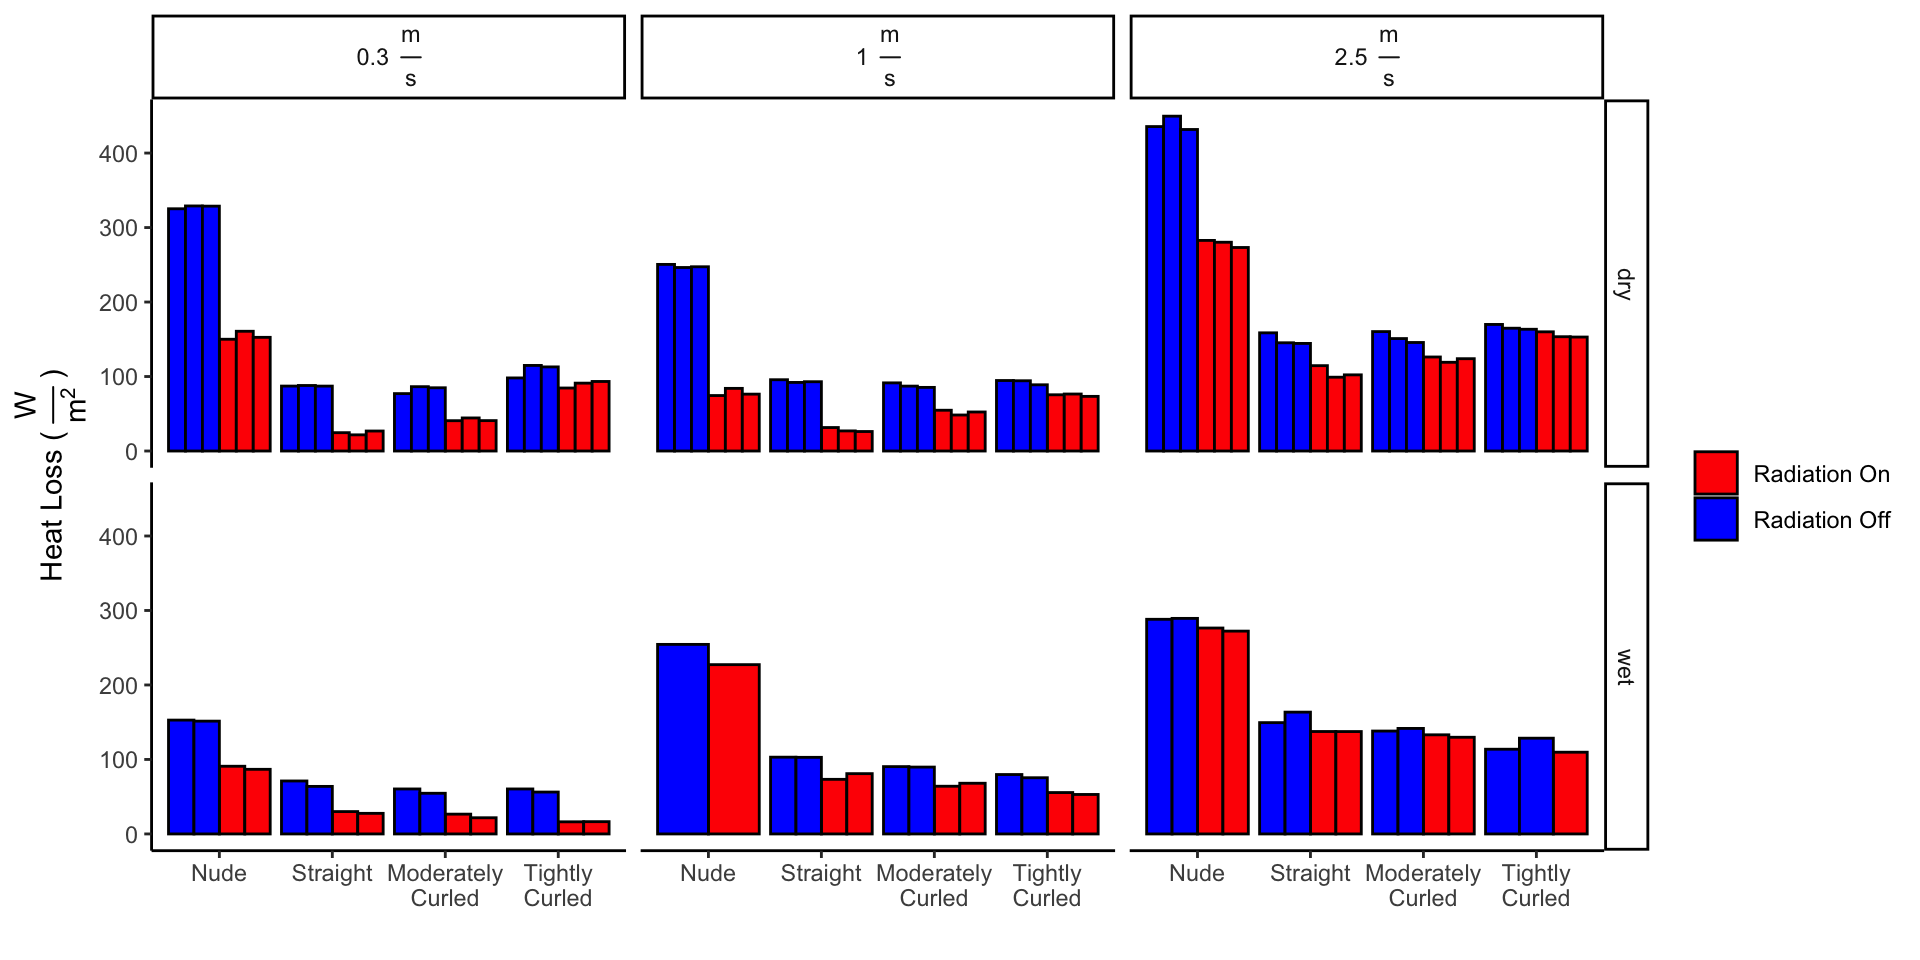
\includegraphics[width=0.95\linewidth]{/Users/tinalasisi-usc/GitHub/HairManikin2023/output/pdf/analysis_files/figure-latex/General-Plots-1}

\hypertarget{removing-outlier}{%
\subsection{Removing Outlier}\label{removing-outlier}}

It was noticed that the 2nd trial conducted with wet, tightly curled
hair, 2.5 m/s wind speed, and radiation on, had more heat loss than any
of the trials with radiation off. With the understanding that radiation
should always decrease heat loss, we elected to remove that data point.

\begin{Shaded}
\begin{Highlighting}[]
\CommentTok{\# Remove specific entry}
\NormalTok{df\_wetdry }\OtherTok{\textless{}{-}}\NormalTok{ df\_wetdry }\SpecialCharTok{\%\textgreater{}\%}
    \FunctionTok{filter}\NormalTok{(}\SpecialCharTok{!}\NormalTok{(wig }\SpecialCharTok{==} \StringTok{"Tightly}\SpecialCharTok{\textbackslash{}n}\StringTok{Curled"} \SpecialCharTok{\&}\NormalTok{ wind }\SpecialCharTok{==} \FloatTok{2.5} \SpecialCharTok{\&}\NormalTok{ radiation }\SpecialCharTok{==}
        \StringTok{"on"} \SpecialCharTok{\&}\NormalTok{ wet\_dry }\SpecialCharTok{==} \StringTok{"wet"} \SpecialCharTok{\&}\NormalTok{ trial }\SpecialCharTok{==} \StringTok{"1"}\NormalTok{))}
\end{Highlighting}
\end{Shaded}

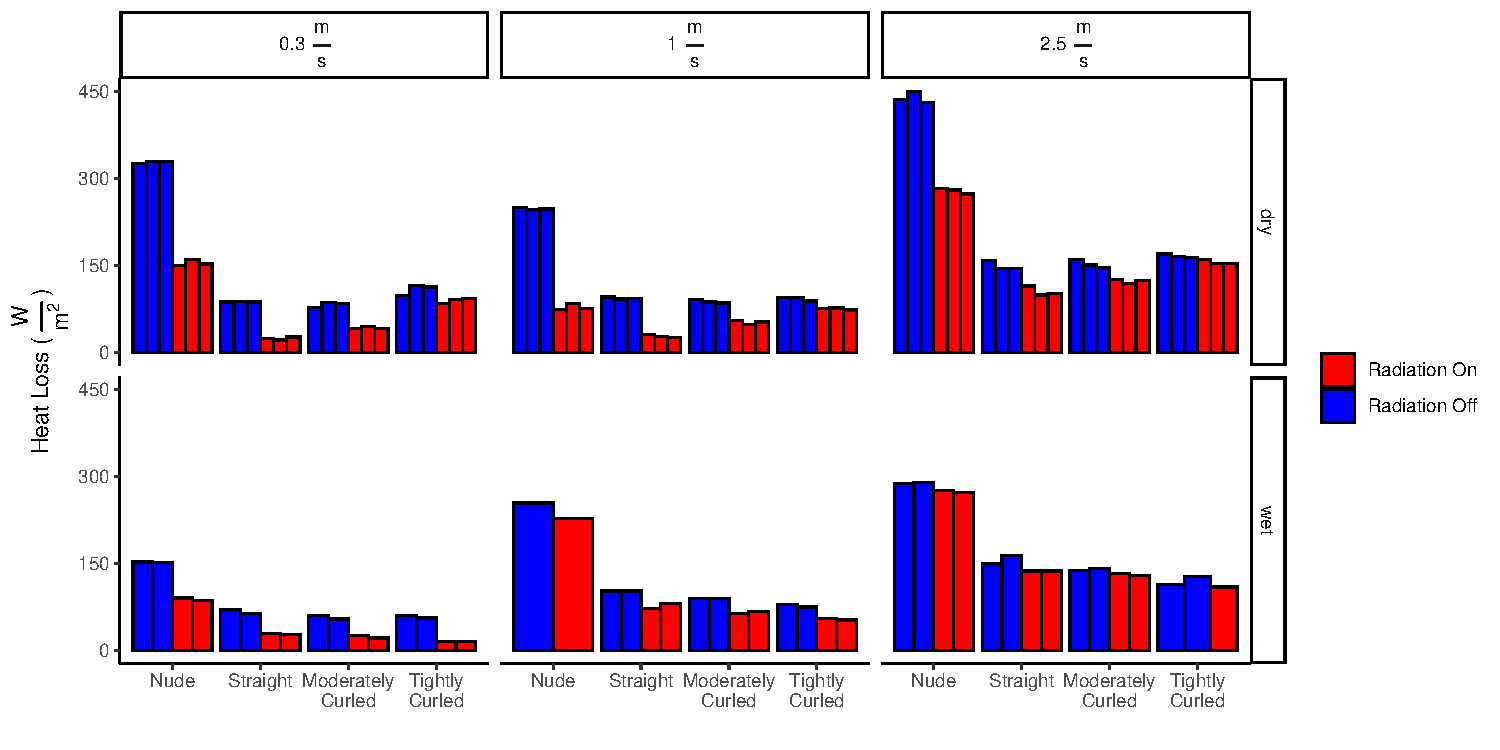
\includegraphics[width=0.95\linewidth]{/Users/tinalasisi-usc/GitHub/HairManikin2023/output/pdf/analysis_files/figure-latex/General-After-Outlier-Removal-1}

\hypertarget{regression-models}{%
\section{Regression models}\label{regression-models}}

\hypertarget{radiation-off}{%
\subsubsection{Radiation off}\label{radiation-off}}

Here, we model the effect of the \texttt{wig} variable on the
\texttt{off} (heat loss without radiation) variable while correcting for
\texttt{wind}.

Without radiation, having hair will reduce the heat loss.

\begin{verbatim}
## 
## Call:
## lm(formula = off ~ wind + wig, data = df_dry_off)
## 
## Residuals:
##     Min      1Q  Median      3Q     Max 
## -8.0303 -3.9809  0.1861  2.6542 14.6310 
## 
## Coefficients:
##                       Estimate Std. Error t value Pr(>|t|)    
## (Intercept)             46.156      2.250   20.52  < 2e-16 ***
## wind                    11.270      1.009   11.17 2.13e-12 ***
## wigStraight            -40.341      2.618  -15.41 4.46e-16 ***
## wigModerately\nCurled  -40.747      2.618  -15.56 3.38e-16 ***
## wigTightly\nCurled     -38.362      2.618  -14.65 1.76e-15 ***
## ---
## Signif. codes:  0 '***' 0.001 '**' 0.01 '*' 0.05 '.' 0.1 ' ' 1
## 
## Residual standard error: 5.555 on 31 degrees of freedom
## Multiple R-squared:  0.9384, Adjusted R-squared:  0.9305 
## F-statistic: 118.1 on 4 and 31 DF,  p-value: < 2.2e-16
\end{verbatim}

\hypertarget{radiation-on}{%
\subsubsection{Radiation on}\label{radiation-on}}

With radiation, there is a net increase in heat (i.e.~heat gain) without
any hair. Additonally, we observe that heat gain decreases with
increasingly curled hair.

\begin{verbatim}
## 
## Call:
## lm(formula = on ~ wind + wig, data = df_dry_on)
## 
## Residuals:
##      Min       1Q   Median       3Q      Max 
## -13.6776  -4.8542  -0.0306   3.3559  19.1058 
## 
## Coefficients:
##                       Estimate Std. Error t value Pr(>|t|)    
## (Intercept)           -129.327      2.835  -45.61  < 2e-16 ***
## wind                    17.406      1.271   13.69  1.1e-14 ***
## wigStraight             69.844      3.300   21.16  < 2e-16 ***
## wigModerately\nCurled   91.558      3.300   27.74  < 2e-16 ***
## wigTightly\nCurled     113.668      3.300   34.44  < 2e-16 ***
## ---
## Signif. codes:  0 '***' 0.001 '**' 0.01 '*' 0.05 '.' 0.1 ' ' 1
## 
## Residual standard error: 7.001 on 31 degrees of freedom
## Multiple R-squared:   0.98,  Adjusted R-squared:  0.9775 
## F-statistic: 380.4 on 4 and 31 DF,  p-value: < 2.2e-16
\end{verbatim}

\hypertarget{solar-influx}{%
\subsubsection{Solar influx}\label{solar-influx}}

Here, we model the effect of the \texttt{wig} variable on
\texttt{influx} while correcting for \texttt{wind}.

In the dry heat loss experiments, we see that all hair (regardless of
curliness) decreases the solar influx. Additionally, the curlier the
hair, the lower the solar influx.

\begin{verbatim}
## 
## Call:
## lm(formula = influx ~ wind + wig, data = df_dry)
## 
## Residuals:
##    Min     1Q Median     3Q    Max 
## -8.079 -3.816  1.087  2.763  9.105 
## 
## Coefficients:
##                        Estimate Std. Error t value Pr(>|t|)    
## (Intercept)            175.4829     2.0133  87.161  < 2e-16 ***
## wind                    -6.1369     0.9028  -6.798  1.3e-07 ***
## wigStraight           -110.1848     2.3434 -47.019  < 2e-16 ***
## wigModerately\nCurled -132.3051     2.3434 -56.459  < 2e-16 ***
## wigTightly\nCurled    -152.0302     2.3434 -64.876  < 2e-16 ***
## ---
## Signif. codes:  0 '***' 0.001 '**' 0.01 '*' 0.05 '.' 0.1 ' ' 1
## 
## Residual standard error: 4.971 on 31 degrees of freedom
## Multiple R-squared:  0.9939, Adjusted R-squared:  0.9932 
## F-statistic:  1272 on 4 and 31 DF,  p-value: < 2.2e-16
\end{verbatim}

\hypertarget{summary-of-dry-heat-loss-regression-models}{%
\subsubsection{Summary of dry heat loss regression
models}\label{summary-of-dry-heat-loss-regression-models}}

 
  \providecommand{\huxb}[2]{\arrayrulecolor[RGB]{#1}\global\arrayrulewidth=#2pt}
  \providecommand{\huxvb}[2]{\color[RGB]{#1}\vrule width #2pt}
  \providecommand{\huxtpad}[1]{\rule{0pt}{#1}}
  \providecommand{\huxbpad}[1]{\rule[-#1]{0pt}{#1}}

\begin{table}[ht]
\begin{centerbox}
\begin{threeparttable}
 \label{tab:lm-summary}
\setlength{\tabcolsep}{0pt}
\begin{tabular}{l l l l}


\hhline{>{\huxb{0, 0, 0}{0.8}}->{\huxb{0, 0, 0}{0.8}}->{\huxb{0, 0, 0}{0.8}}->{\huxb{0, 0, 0}{0.8}}-}
\arrayrulecolor{black}

\multicolumn{1}{!{\huxvb{0, 0, 0}{0}}c!{\huxvb{0, 0, 0}{0}}}{\huxtpad{6pt + 1em}\centering \hspace{6pt}  \hspace{6pt}\huxbpad{6pt}} &
\multicolumn{1}{c!{\huxvb{0, 0, 0}{0}}}{\huxtpad{6pt + 1em}\centering \hspace{6pt} Radiation Off \hspace{6pt}\huxbpad{6pt}} &
\multicolumn{1}{c!{\huxvb{0, 0, 0}{0}}}{\huxtpad{6pt + 1em}\centering \hspace{6pt} Radiation On \hspace{6pt}\huxbpad{6pt}} &
\multicolumn{1}{c!{\huxvb{0, 0, 0}{0}}}{\huxtpad{6pt + 1em}\centering \hspace{6pt} Solar Influx \hspace{6pt}\huxbpad{6pt}} \tabularnewline[-0.5pt]


\hhline{>{\huxb{255, 255, 255}{0.4}}->{\huxb{0, 0, 0}{0.4}}->{\huxb{0, 0, 0}{0.4}}->{\huxb{0, 0, 0}{0.4}}-}
\arrayrulecolor{black}

\multicolumn{1}{!{\huxvb{0, 0, 0}{0}}l!{\huxvb{0, 0, 0}{0}}}{\huxtpad{6pt + 1em}\raggedright \hspace{6pt} (Intercept) \hspace{6pt}\huxbpad{6pt}} &
\multicolumn{1}{r!{\huxvb{0, 0, 0}{0}}}{\huxtpad{6pt + 1em}\raggedleft \hspace{6pt} 46.16 *** \hspace{6pt}\huxbpad{6pt}} &
\multicolumn{1}{r!{\huxvb{0, 0, 0}{0}}}{\huxtpad{6pt + 1em}\raggedleft \hspace{6pt} -129.33 *** \hspace{6pt}\huxbpad{6pt}} &
\multicolumn{1}{r!{\huxvb{0, 0, 0}{0}}}{\huxtpad{6pt + 1em}\raggedleft \hspace{6pt} 175.48 *** \hspace{6pt}\huxbpad{6pt}} \tabularnewline[-0.5pt]


\hhline{}
\arrayrulecolor{black}

\multicolumn{1}{!{\huxvb{0, 0, 0}{0}}l!{\huxvb{0, 0, 0}{0}}}{\huxtpad{6pt + 1em}\raggedright \hspace{6pt}  \hspace{6pt}\huxbpad{6pt}} &
\multicolumn{1}{r!{\huxvb{0, 0, 0}{0}}}{\huxtpad{6pt + 1em}\raggedleft \hspace{6pt} [41.57, 50.74]\hphantom{0}\hphantom{0}\hphantom{0} \hspace{6pt}\huxbpad{6pt}} &
\multicolumn{1}{r!{\huxvb{0, 0, 0}{0}}}{\huxtpad{6pt + 1em}\raggedleft \hspace{6pt} [-135.11, -123.54]\hphantom{0}\hphantom{0}\hphantom{0} \hspace{6pt}\huxbpad{6pt}} &
\multicolumn{1}{r!{\huxvb{0, 0, 0}{0}}}{\huxtpad{6pt + 1em}\raggedleft \hspace{6pt} [171.38, 179.59]\hphantom{0}\hphantom{0}\hphantom{0} \hspace{6pt}\huxbpad{6pt}} \tabularnewline[-0.5pt]


\hhline{}
\arrayrulecolor{black}

\multicolumn{1}{!{\huxvb{0, 0, 0}{0}}l!{\huxvb{0, 0, 0}{0}}}{\huxtpad{6pt + 1em}\raggedright \hspace{6pt} wind \hspace{6pt}\huxbpad{6pt}} &
\multicolumn{1}{r!{\huxvb{0, 0, 0}{0}}}{\huxtpad{6pt + 1em}\raggedleft \hspace{6pt} 11.27 *** \hspace{6pt}\huxbpad{6pt}} &
\multicolumn{1}{r!{\huxvb{0, 0, 0}{0}}}{\huxtpad{6pt + 1em}\raggedleft \hspace{6pt} 17.41 *** \hspace{6pt}\huxbpad{6pt}} &
\multicolumn{1}{r!{\huxvb{0, 0, 0}{0}}}{\huxtpad{6pt + 1em}\raggedleft \hspace{6pt} -6.14 *** \hspace{6pt}\huxbpad{6pt}} \tabularnewline[-0.5pt]


\hhline{}
\arrayrulecolor{black}

\multicolumn{1}{!{\huxvb{0, 0, 0}{0}}l!{\huxvb{0, 0, 0}{0}}}{\huxtpad{6pt + 1em}\raggedright \hspace{6pt}  \hspace{6pt}\huxbpad{6pt}} &
\multicolumn{1}{r!{\huxvb{0, 0, 0}{0}}}{\huxtpad{6pt + 1em}\raggedleft \hspace{6pt} [9.21, 13.33]\hphantom{0}\hphantom{0}\hphantom{0} \hspace{6pt}\huxbpad{6pt}} &
\multicolumn{1}{r!{\huxvb{0, 0, 0}{0}}}{\huxtpad{6pt + 1em}\raggedleft \hspace{6pt} [14.81, 20.00]\hphantom{0}\hphantom{0}\hphantom{0} \hspace{6pt}\huxbpad{6pt}} &
\multicolumn{1}{r!{\huxvb{0, 0, 0}{0}}}{\huxtpad{6pt + 1em}\raggedleft \hspace{6pt} [-7.98, -4.30]\hphantom{0}\hphantom{0}\hphantom{0} \hspace{6pt}\huxbpad{6pt}} \tabularnewline[-0.5pt]


\hhline{}
\arrayrulecolor{black}

\multicolumn{1}{!{\huxvb{0, 0, 0}{0}}l!{\huxvb{0, 0, 0}{0}}}{\huxtpad{6pt + 1em}\raggedright \hspace{6pt} wigStraight \hspace{6pt}\huxbpad{6pt}} &
\multicolumn{1}{r!{\huxvb{0, 0, 0}{0}}}{\huxtpad{6pt + 1em}\raggedleft \hspace{6pt} -40.34 *** \hspace{6pt}\huxbpad{6pt}} &
\multicolumn{1}{r!{\huxvb{0, 0, 0}{0}}}{\huxtpad{6pt + 1em}\raggedleft \hspace{6pt} 69.84 *** \hspace{6pt}\huxbpad{6pt}} &
\multicolumn{1}{r!{\huxvb{0, 0, 0}{0}}}{\huxtpad{6pt + 1em}\raggedleft \hspace{6pt} -110.18 *** \hspace{6pt}\huxbpad{6pt}} \tabularnewline[-0.5pt]


\hhline{}
\arrayrulecolor{black}

\multicolumn{1}{!{\huxvb{0, 0, 0}{0}}l!{\huxvb{0, 0, 0}{0}}}{\huxtpad{6pt + 1em}\raggedright \hspace{6pt}  \hspace{6pt}\huxbpad{6pt}} &
\multicolumn{1}{r!{\huxvb{0, 0, 0}{0}}}{\huxtpad{6pt + 1em}\raggedleft \hspace{6pt} [-45.68, -35.00]\hphantom{0}\hphantom{0}\hphantom{0} \hspace{6pt}\huxbpad{6pt}} &
\multicolumn{1}{r!{\huxvb{0, 0, 0}{0}}}{\huxtpad{6pt + 1em}\raggedleft \hspace{6pt} [63.11, 76.58]\hphantom{0}\hphantom{0}\hphantom{0} \hspace{6pt}\huxbpad{6pt}} &
\multicolumn{1}{r!{\huxvb{0, 0, 0}{0}}}{\huxtpad{6pt + 1em}\raggedleft \hspace{6pt} [-114.96, -105.41]\hphantom{0}\hphantom{0}\hphantom{0} \hspace{6pt}\huxbpad{6pt}} \tabularnewline[-0.5pt]


\hhline{}
\arrayrulecolor{black}

\multicolumn{1}{!{\huxvb{0, 0, 0}{0}}l!{\huxvb{0, 0, 0}{0}}}{\huxtpad{6pt + 1em}\raggedright \hspace{6pt} wigModerately \newline Curled \hspace{6pt}\huxbpad{6pt}} &
\multicolumn{1}{r!{\huxvb{0, 0, 0}{0}}}{\huxtpad{6pt + 1em}\raggedleft \hspace{6pt} -40.75 *** \hspace{6pt}\huxbpad{6pt}} &
\multicolumn{1}{r!{\huxvb{0, 0, 0}{0}}}{\huxtpad{6pt + 1em}\raggedleft \hspace{6pt} 91.56 *** \hspace{6pt}\huxbpad{6pt}} &
\multicolumn{1}{r!{\huxvb{0, 0, 0}{0}}}{\huxtpad{6pt + 1em}\raggedleft \hspace{6pt} -132.31 *** \hspace{6pt}\huxbpad{6pt}} \tabularnewline[-0.5pt]


\hhline{}
\arrayrulecolor{black}

\multicolumn{1}{!{\huxvb{0, 0, 0}{0}}l!{\huxvb{0, 0, 0}{0}}}{\huxtpad{6pt + 1em}\raggedright \hspace{6pt}  \hspace{6pt}\huxbpad{6pt}} &
\multicolumn{1}{r!{\huxvb{0, 0, 0}{0}}}{\huxtpad{6pt + 1em}\raggedleft \hspace{6pt} [-46.09, -35.41]\hphantom{0}\hphantom{0}\hphantom{0} \hspace{6pt}\huxbpad{6pt}} &
\multicolumn{1}{r!{\huxvb{0, 0, 0}{0}}}{\huxtpad{6pt + 1em}\raggedleft \hspace{6pt} [84.83, 98.29]\hphantom{0}\hphantom{0}\hphantom{0} \hspace{6pt}\huxbpad{6pt}} &
\multicolumn{1}{r!{\huxvb{0, 0, 0}{0}}}{\huxtpad{6pt + 1em}\raggedleft \hspace{6pt} [-137.08, -127.53]\hphantom{0}\hphantom{0}\hphantom{0} \hspace{6pt}\huxbpad{6pt}} \tabularnewline[-0.5pt]


\hhline{}
\arrayrulecolor{black}

\multicolumn{1}{!{\huxvb{0, 0, 0}{0}}l!{\huxvb{0, 0, 0}{0}}}{\huxtpad{6pt + 1em}\raggedright \hspace{6pt} wigTightly \newline Curled \hspace{6pt}\huxbpad{6pt}} &
\multicolumn{1}{r!{\huxvb{0, 0, 0}{0}}}{\huxtpad{6pt + 1em}\raggedleft \hspace{6pt} -38.36 *** \hspace{6pt}\huxbpad{6pt}} &
\multicolumn{1}{r!{\huxvb{0, 0, 0}{0}}}{\huxtpad{6pt + 1em}\raggedleft \hspace{6pt} 113.67 *** \hspace{6pt}\huxbpad{6pt}} &
\multicolumn{1}{r!{\huxvb{0, 0, 0}{0}}}{\huxtpad{6pt + 1em}\raggedleft \hspace{6pt} -152.03 *** \hspace{6pt}\huxbpad{6pt}} \tabularnewline[-0.5pt]


\hhline{}
\arrayrulecolor{black}

\multicolumn{1}{!{\huxvb{0, 0, 0}{0}}l!{\huxvb{0, 0, 0}{0}}}{\huxtpad{6pt + 1em}\raggedright \hspace{6pt}  \hspace{6pt}\huxbpad{6pt}} &
\multicolumn{1}{r!{\huxvb{0, 0, 0}{0}}}{\huxtpad{6pt + 1em}\raggedleft \hspace{6pt} [-43.70, -33.02]\hphantom{0}\hphantom{0}\hphantom{0} \hspace{6pt}\huxbpad{6pt}} &
\multicolumn{1}{r!{\huxvb{0, 0, 0}{0}}}{\huxtpad{6pt + 1em}\raggedleft \hspace{6pt} [106.94, 120.40]\hphantom{0}\hphantom{0}\hphantom{0} \hspace{6pt}\huxbpad{6pt}} &
\multicolumn{1}{r!{\huxvb{0, 0, 0}{0}}}{\huxtpad{6pt + 1em}\raggedleft \hspace{6pt} [-156.81, -147.25]\hphantom{0}\hphantom{0}\hphantom{0} \hspace{6pt}\huxbpad{6pt}} \tabularnewline[-0.5pt]


\hhline{>{\huxb{255, 255, 255}{0.4}}->{\huxb{0, 0, 0}{0.4}}->{\huxb{0, 0, 0}{0.4}}->{\huxb{0, 0, 0}{0.4}}-}
\arrayrulecolor{black}

\multicolumn{1}{!{\huxvb{0, 0, 0}{0}}l!{\huxvb{0, 0, 0}{0}}}{\huxtpad{6pt + 1em}\raggedright \hspace{6pt} N \hspace{6pt}\huxbpad{6pt}} &
\multicolumn{1}{r!{\huxvb{0, 0, 0}{0}}}{\huxtpad{6pt + 1em}\raggedleft \hspace{6pt} 36\hphantom{0}\hphantom{0}\hphantom{0}\hphantom{0}\hphantom{0}\hphantom{0}\hphantom{0} \hspace{6pt}\huxbpad{6pt}} &
\multicolumn{1}{r!{\huxvb{0, 0, 0}{0}}}{\huxtpad{6pt + 1em}\raggedleft \hspace{6pt} 36\hphantom{0}\hphantom{0}\hphantom{0}\hphantom{0}\hphantom{0}\hphantom{0}\hphantom{0} \hspace{6pt}\huxbpad{6pt}} &
\multicolumn{1}{r!{\huxvb{0, 0, 0}{0}}}{\huxtpad{6pt + 1em}\raggedleft \hspace{6pt} 36\hphantom{0}\hphantom{0}\hphantom{0}\hphantom{0}\hphantom{0}\hphantom{0}\hphantom{0} \hspace{6pt}\huxbpad{6pt}} \tabularnewline[-0.5pt]


\hhline{}
\arrayrulecolor{black}

\multicolumn{1}{!{\huxvb{0, 0, 0}{0}}l!{\huxvb{0, 0, 0}{0}}}{\huxtpad{6pt + 1em}\raggedright \hspace{6pt} R2 \hspace{6pt}\huxbpad{6pt}} &
\multicolumn{1}{r!{\huxvb{0, 0, 0}{0}}}{\huxtpad{6pt + 1em}\raggedleft \hspace{6pt} 0.94\hphantom{0}\hphantom{0}\hphantom{0}\hphantom{0} \hspace{6pt}\huxbpad{6pt}} &
\multicolumn{1}{r!{\huxvb{0, 0, 0}{0}}}{\huxtpad{6pt + 1em}\raggedleft \hspace{6pt} 0.98\hphantom{0}\hphantom{0}\hphantom{0}\hphantom{0} \hspace{6pt}\huxbpad{6pt}} &
\multicolumn{1}{r!{\huxvb{0, 0, 0}{0}}}{\huxtpad{6pt + 1em}\raggedleft \hspace{6pt} 0.99\hphantom{0}\hphantom{0}\hphantom{0}\hphantom{0} \hspace{6pt}\huxbpad{6pt}} \tabularnewline[-0.5pt]


\hhline{>{\huxb{0, 0, 0}{0.8}}->{\huxb{0, 0, 0}{0.8}}->{\huxb{0, 0, 0}{0.8}}->{\huxb{0, 0, 0}{0.8}}-}
\arrayrulecolor{black}

\multicolumn{4}{!{\huxvb{0, 0, 0}{0}}l!{\huxvb{0, 0, 0}{0}}}{\huxtpad{6pt + 1em}\raggedright \hspace{6pt}  *** p $<$ 0.001;  ** p $<$ 0.01;  * p $<$ 0.05. \hspace{6pt}\huxbpad{6pt}} \tabularnewline[-0.5pt]


\hhline{}
\arrayrulecolor{black}
\end{tabular}
\end{threeparttable}\par\end{centerbox}

\end{table}
 

\begin{figure}

{\centering 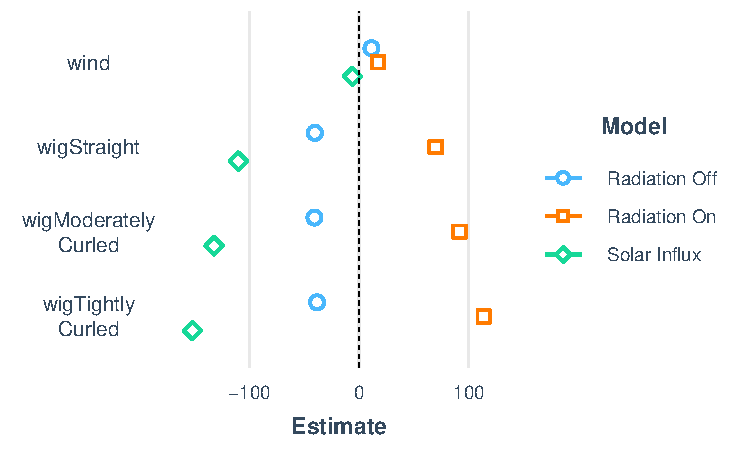
\includegraphics[width=0.6\linewidth]{/Users/tinalasisi-usc/GitHub/HairManikin2023/output/pdf/analysis_files/figure-latex/plt-summary-models-1} 

}

\caption{Regression coefficients across regression models.}\label{fig:plt-summary-models}
\end{figure}

\hypertarget{dry-heat-loss-anova-plots}{%
\subsubsection{Dry heat loss ANOVA
plots}\label{dry-heat-loss-anova-plots}}

\begin{figure}

{\centering 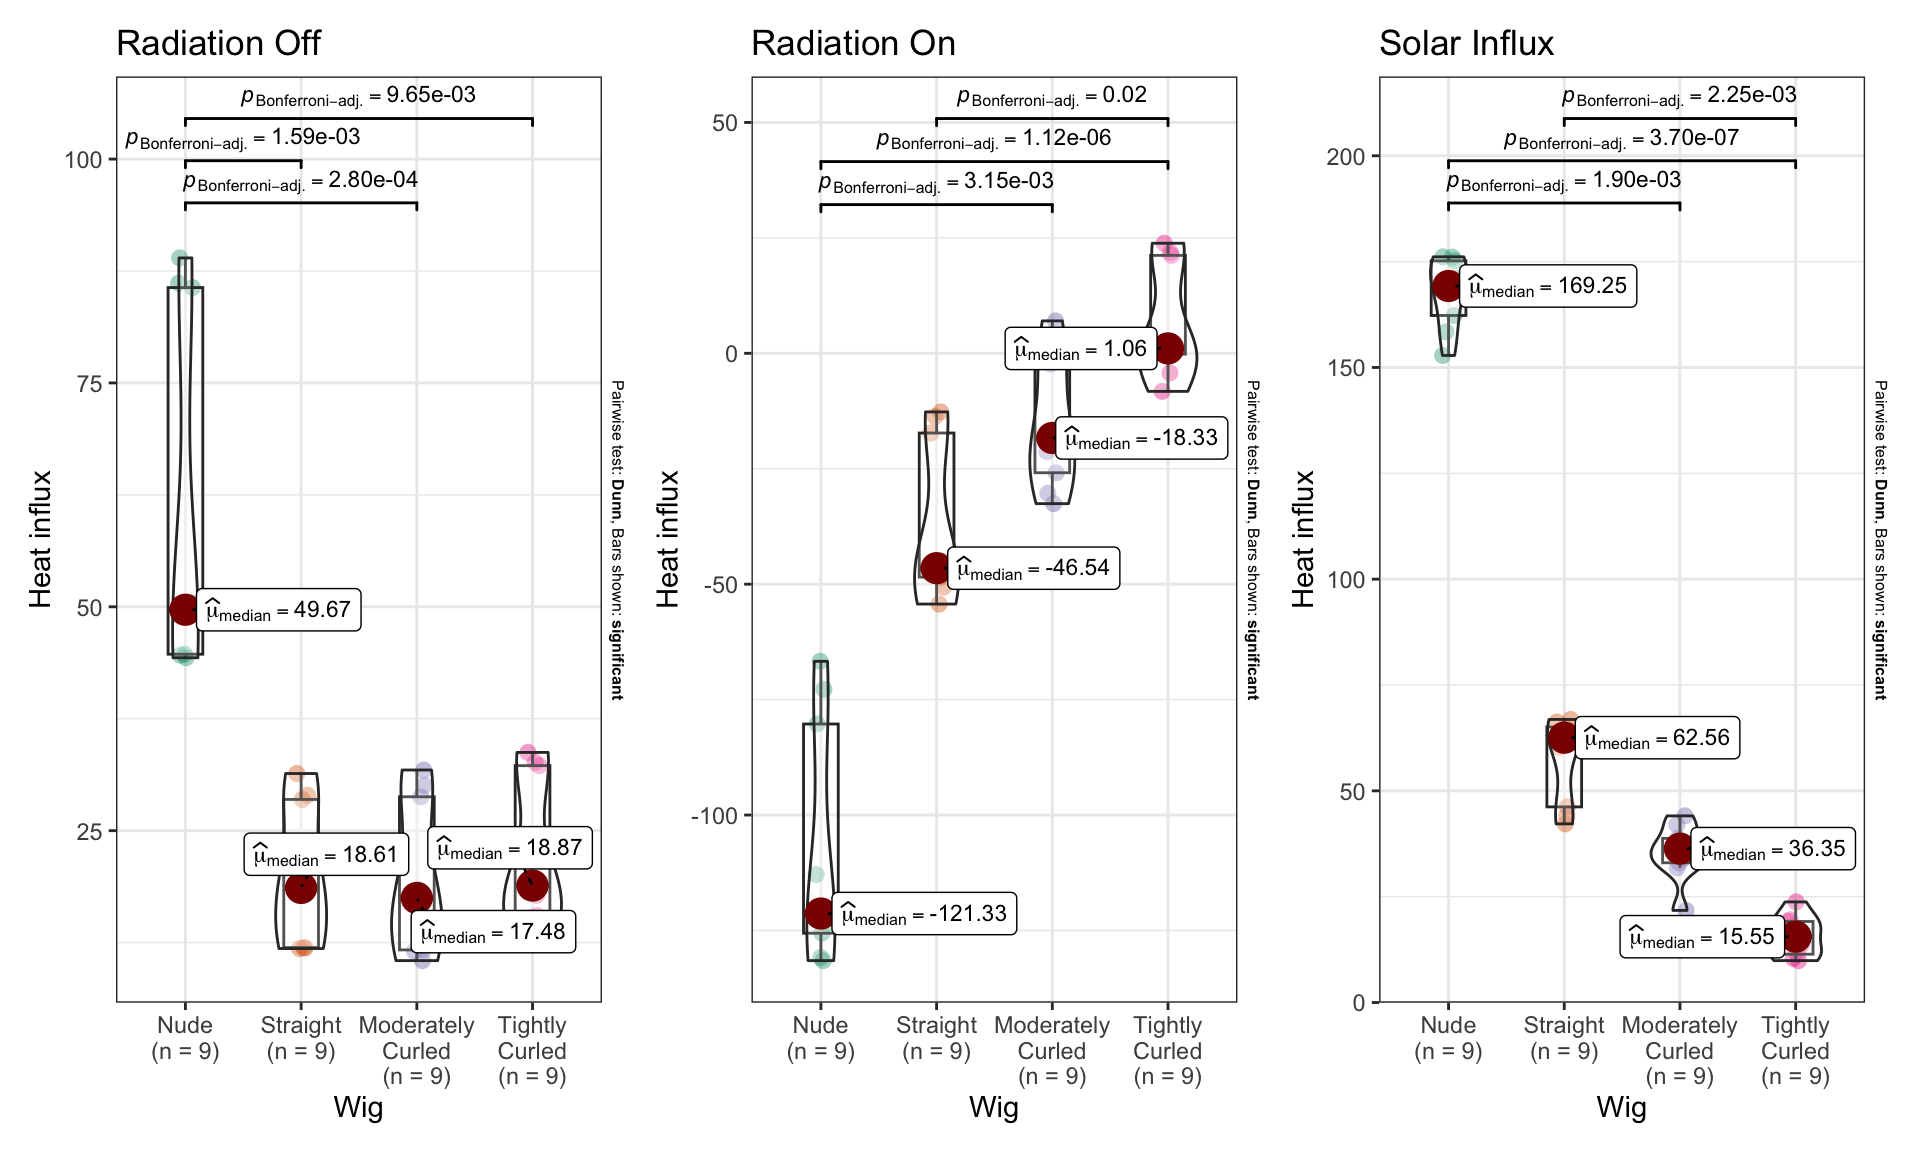
\includegraphics[width=0.95\linewidth]{/Users/tinalasisi-usc/GitHub/HairManikin2023/output/pdf/analysis_files/figure-latex/ggbetweenstats-dry-1} 

}

\caption{ANOVA of dry heat loss}\label{fig:ggbetweenstats-dry}
\end{figure}

\hypertarget{evaporative-resistance-wet-experiments}{%
\subsection{Evaporative resistance (wet
experiments)}\label{evaporative-resistance-wet-experiments}}

Here, we repeat the same modelling process for the evaporative
resistance data from the wet experiments.

\hypertarget{radiation-off-1}{%
\subsubsection{Radiation off}\label{radiation-off-1}}

Here, we model the effect of the \texttt{wig} variable on the
\texttt{off} (heat loss without radiation) variable while correcting for
\texttt{wind}.

Without solar radiation, all hair (regardless of texture) decreases
evaporative resistance.

\begin{verbatim}
## 
## Call:
## lm(formula = off ~ wind + wig, data = df_wet_off)
## 
## Residuals:
##     Min      1Q  Median      3Q     Max 
## -32.382  -6.006   2.673   5.870  40.839 
## 
## Coefficients:
##                       Estimate Std. Error t value Pr(>|t|)    
## (Intercept)            171.043      9.132   18.73 8.71e-13 ***
## wind                    42.585      3.929   10.84 4.69e-09 ***
## wigStraight           -116.024     10.179  -11.40 2.20e-09 ***
## wigModerately\nCurled -129.170     10.179  -12.69 4.26e-10 ***
## wigTightly\nCurled    -134.409     10.695  -12.57 4.95e-10 ***
## ---
## Signif. codes:  0 '***' 0.001 '**' 0.01 '*' 0.05 '.' 0.1 ' ' 1
## 
## Residual standard error: 16.81 on 17 degrees of freedom
## Multiple R-squared:  0.9551, Adjusted R-squared:  0.9446 
## F-statistic: 90.46 on 4 and 17 DF,  p-value: 3.177e-11
\end{verbatim}

\hypertarget{radiation-on-1}{%
\subsubsection{Radiation on}\label{radiation-on-1}}

With radiation, hair decreases evaporative resistance.

\begin{verbatim}
## 
## Call:
## lm(formula = on ~ wind + wig, data = df_wet_on)
## 
## Residuals:
##     Min      1Q  Median      3Q     Max 
## -47.426 -11.303   4.423   6.822  54.290 
## 
## Coefficients:
##                       Estimate Std. Error t value Pr(>|t|)    
## (Intercept)            117.541     12.726   9.236 4.90e-08 ***
## wind                    55.445      5.475  10.127 1.29e-08 ***
## wigStraight           -106.632     14.186  -7.517 8.44e-07 ***
## wigModerately\nCurled -113.898     14.186  -8.029 3.48e-07 ***
## wigTightly\nCurled    -123.891     14.905  -8.312 2.16e-07 ***
## ---
## Signif. codes:  0 '***' 0.001 '**' 0.01 '*' 0.05 '.' 0.1 ' ' 1
## 
## Residual standard error: 23.42 on 17 degrees of freedom
## Multiple R-squared:  0.9255, Adjusted R-squared:  0.908 
## F-statistic:  52.8 on 4 and 17 DF,  p-value: 2.297e-09
\end{verbatim}

\hypertarget{solar-influx-1}{%
\subsubsection{Solar influx}\label{solar-influx-1}}

Combining the above data to calculate solar influx, we see that there is
not a considerable effect of radiation on evaporative resistance.

\begin{verbatim}
## 
## Call:
## lm(formula = influx ~ wind + wig, data = df_wet)
## 
## Residuals:
##      Min       1Q   Median       3Q      Max 
## -13.4512  -4.2205  -0.7951   3.9758  15.0438 
## 
## Coefficients:
##                       Estimate Std. Error t value Pr(>|t|)    
## (Intercept)             53.502      4.585  11.669 1.54e-09 ***
## wind                   -12.860      1.973  -6.520 5.24e-06 ***
## wigStraight             -9.392      5.111  -1.838  0.08368 .  
## wigModerately\nCurled  -15.272      5.111  -2.988  0.00826 ** 
## wigTightly\nCurled     -10.518      5.370  -1.959  0.06676 .  
## ---
## Signif. codes:  0 '***' 0.001 '**' 0.01 '*' 0.05 '.' 0.1 ' ' 1
## 
## Residual standard error: 8.439 on 17 degrees of freedom
## Multiple R-squared:  0.7493, Adjusted R-squared:  0.6903 
## F-statistic:  12.7 on 4 and 17 DF,  p-value: 5.753e-05
\end{verbatim}

\hypertarget{summary-of-evaporative-heat-loss-regression-models}{%
\subsubsection{Summary of evaporative heat loss regression
models}\label{summary-of-evaporative-heat-loss-regression-models}}

 
  \providecommand{\huxb}[2]{\arrayrulecolor[RGB]{#1}\global\arrayrulewidth=#2pt}
  \providecommand{\huxvb}[2]{\color[RGB]{#1}\vrule width #2pt}
  \providecommand{\huxtpad}[1]{\rule{0pt}{#1}}
  \providecommand{\huxbpad}[1]{\rule[-#1]{0pt}{#1}}

\begin{table}[ht]
\begin{centerbox}
\begin{threeparttable}
 \label{tab:lm-summary-wet}
\setlength{\tabcolsep}{0pt}
\begin{tabular}{l l l l}


\hhline{>{\huxb{0, 0, 0}{0.8}}->{\huxb{0, 0, 0}{0.8}}->{\huxb{0, 0, 0}{0.8}}->{\huxb{0, 0, 0}{0.8}}-}
\arrayrulecolor{black}

\multicolumn{1}{!{\huxvb{0, 0, 0}{0}}c!{\huxvb{0, 0, 0}{0}}}{\huxtpad{6pt + 1em}\centering \hspace{6pt}  \hspace{6pt}\huxbpad{6pt}} &
\multicolumn{1}{c!{\huxvb{0, 0, 0}{0}}}{\huxtpad{6pt + 1em}\centering \hspace{6pt} Radiation Off \hspace{6pt}\huxbpad{6pt}} &
\multicolumn{1}{c!{\huxvb{0, 0, 0}{0}}}{\huxtpad{6pt + 1em}\centering \hspace{6pt} Radiation On \hspace{6pt}\huxbpad{6pt}} &
\multicolumn{1}{c!{\huxvb{0, 0, 0}{0}}}{\huxtpad{6pt + 1em}\centering \hspace{6pt} Solar Influx \hspace{6pt}\huxbpad{6pt}} \tabularnewline[-0.5pt]


\hhline{>{\huxb{255, 255, 255}{0.4}}->{\huxb{0, 0, 0}{0.4}}->{\huxb{0, 0, 0}{0.4}}->{\huxb{0, 0, 0}{0.4}}-}
\arrayrulecolor{black}

\multicolumn{1}{!{\huxvb{0, 0, 0}{0}}l!{\huxvb{0, 0, 0}{0}}}{\huxtpad{6pt + 1em}\raggedright \hspace{6pt} (Intercept) \hspace{6pt}\huxbpad{6pt}} &
\multicolumn{1}{r!{\huxvb{0, 0, 0}{0}}}{\huxtpad{6pt + 1em}\raggedleft \hspace{6pt} 171.04 *** \hspace{6pt}\huxbpad{6pt}} &
\multicolumn{1}{r!{\huxvb{0, 0, 0}{0}}}{\huxtpad{6pt + 1em}\raggedleft \hspace{6pt} 117.54 *** \hspace{6pt}\huxbpad{6pt}} &
\multicolumn{1}{r!{\huxvb{0, 0, 0}{0}}}{\huxtpad{6pt + 1em}\raggedleft \hspace{6pt} 53.50 *** \hspace{6pt}\huxbpad{6pt}} \tabularnewline[-0.5pt]


\hhline{}
\arrayrulecolor{black}

\multicolumn{1}{!{\huxvb{0, 0, 0}{0}}l!{\huxvb{0, 0, 0}{0}}}{\huxtpad{6pt + 1em}\raggedright \hspace{6pt}  \hspace{6pt}\huxbpad{6pt}} &
\multicolumn{1}{r!{\huxvb{0, 0, 0}{0}}}{\huxtpad{6pt + 1em}\raggedleft \hspace{6pt} [151.78, 190.31]\hphantom{0}\hphantom{0}\hphantom{0} \hspace{6pt}\huxbpad{6pt}} &
\multicolumn{1}{r!{\huxvb{0, 0, 0}{0}}}{\huxtpad{6pt + 1em}\raggedleft \hspace{6pt} [90.69, 144.39]\hphantom{0}\hphantom{0}\hphantom{0} \hspace{6pt}\huxbpad{6pt}} &
\multicolumn{1}{r!{\huxvb{0, 0, 0}{0}}}{\huxtpad{6pt + 1em}\raggedleft \hspace{6pt} [43.83, 63.18]\hphantom{0}\hphantom{0}\hphantom{0} \hspace{6pt}\huxbpad{6pt}} \tabularnewline[-0.5pt]


\hhline{}
\arrayrulecolor{black}

\multicolumn{1}{!{\huxvb{0, 0, 0}{0}}l!{\huxvb{0, 0, 0}{0}}}{\huxtpad{6pt + 1em}\raggedright \hspace{6pt} wind \hspace{6pt}\huxbpad{6pt}} &
\multicolumn{1}{r!{\huxvb{0, 0, 0}{0}}}{\huxtpad{6pt + 1em}\raggedleft \hspace{6pt} 42.58 *** \hspace{6pt}\huxbpad{6pt}} &
\multicolumn{1}{r!{\huxvb{0, 0, 0}{0}}}{\huxtpad{6pt + 1em}\raggedleft \hspace{6pt} 55.44 *** \hspace{6pt}\huxbpad{6pt}} &
\multicolumn{1}{r!{\huxvb{0, 0, 0}{0}}}{\huxtpad{6pt + 1em}\raggedleft \hspace{6pt} -12.86 *** \hspace{6pt}\huxbpad{6pt}} \tabularnewline[-0.5pt]


\hhline{}
\arrayrulecolor{black}

\multicolumn{1}{!{\huxvb{0, 0, 0}{0}}l!{\huxvb{0, 0, 0}{0}}}{\huxtpad{6pt + 1em}\raggedright \hspace{6pt}  \hspace{6pt}\huxbpad{6pt}} &
\multicolumn{1}{r!{\huxvb{0, 0, 0}{0}}}{\huxtpad{6pt + 1em}\raggedleft \hspace{6pt} [34.30, 50.87]\hphantom{0}\hphantom{0}\hphantom{0} \hspace{6pt}\huxbpad{6pt}} &
\multicolumn{1}{r!{\huxvb{0, 0, 0}{0}}}{\huxtpad{6pt + 1em}\raggedleft \hspace{6pt} [43.89, 67.00]\hphantom{0}\hphantom{0}\hphantom{0} \hspace{6pt}\huxbpad{6pt}} &
\multicolumn{1}{r!{\huxvb{0, 0, 0}{0}}}{\huxtpad{6pt + 1em}\raggedleft \hspace{6pt} [-17.02, -8.70]\hphantom{0}\hphantom{0}\hphantom{0} \hspace{6pt}\huxbpad{6pt}} \tabularnewline[-0.5pt]


\hhline{}
\arrayrulecolor{black}

\multicolumn{1}{!{\huxvb{0, 0, 0}{0}}l!{\huxvb{0, 0, 0}{0}}}{\huxtpad{6pt + 1em}\raggedright \hspace{6pt} wigStraight \hspace{6pt}\huxbpad{6pt}} &
\multicolumn{1}{r!{\huxvb{0, 0, 0}{0}}}{\huxtpad{6pt + 1em}\raggedleft \hspace{6pt} -116.02 *** \hspace{6pt}\huxbpad{6pt}} &
\multicolumn{1}{r!{\huxvb{0, 0, 0}{0}}}{\huxtpad{6pt + 1em}\raggedleft \hspace{6pt} -106.63 *** \hspace{6pt}\huxbpad{6pt}} &
\multicolumn{1}{r!{\huxvb{0, 0, 0}{0}}}{\huxtpad{6pt + 1em}\raggedleft \hspace{6pt} -9.39\hphantom{0}\hphantom{0}\hphantom{0}\hphantom{0} \hspace{6pt}\huxbpad{6pt}} \tabularnewline[-0.5pt]


\hhline{}
\arrayrulecolor{black}

\multicolumn{1}{!{\huxvb{0, 0, 0}{0}}l!{\huxvb{0, 0, 0}{0}}}{\huxtpad{6pt + 1em}\raggedright \hspace{6pt}  \hspace{6pt}\huxbpad{6pt}} &
\multicolumn{1}{r!{\huxvb{0, 0, 0}{0}}}{\huxtpad{6pt + 1em}\raggedleft \hspace{6pt} [-137.50, -94.55]\hphantom{0}\hphantom{0}\hphantom{0} \hspace{6pt}\huxbpad{6pt}} &
\multicolumn{1}{r!{\huxvb{0, 0, 0}{0}}}{\huxtpad{6pt + 1em}\raggedleft \hspace{6pt} [-136.56, -76.70]\hphantom{0}\hphantom{0}\hphantom{0} \hspace{6pt}\huxbpad{6pt}} &
\multicolumn{1}{r!{\huxvb{0, 0, 0}{0}}}{\huxtpad{6pt + 1em}\raggedleft \hspace{6pt} [-20.17, 1.39]\hphantom{0}\hphantom{0}\hphantom{0} \hspace{6pt}\huxbpad{6pt}} \tabularnewline[-0.5pt]


\hhline{}
\arrayrulecolor{black}

\multicolumn{1}{!{\huxvb{0, 0, 0}{0}}l!{\huxvb{0, 0, 0}{0}}}{\huxtpad{6pt + 1em}\raggedright \hspace{6pt} wigModerately \newline Curled \hspace{6pt}\huxbpad{6pt}} &
\multicolumn{1}{r!{\huxvb{0, 0, 0}{0}}}{\huxtpad{6pt + 1em}\raggedleft \hspace{6pt} -129.17 *** \hspace{6pt}\huxbpad{6pt}} &
\multicolumn{1}{r!{\huxvb{0, 0, 0}{0}}}{\huxtpad{6pt + 1em}\raggedleft \hspace{6pt} -113.90 *** \hspace{6pt}\huxbpad{6pt}} &
\multicolumn{1}{r!{\huxvb{0, 0, 0}{0}}}{\huxtpad{6pt + 1em}\raggedleft \hspace{6pt} -15.27 **\hphantom{0} \hspace{6pt}\huxbpad{6pt}} \tabularnewline[-0.5pt]


\hhline{}
\arrayrulecolor{black}

\multicolumn{1}{!{\huxvb{0, 0, 0}{0}}l!{\huxvb{0, 0, 0}{0}}}{\huxtpad{6pt + 1em}\raggedright \hspace{6pt}  \hspace{6pt}\huxbpad{6pt}} &
\multicolumn{1}{r!{\huxvb{0, 0, 0}{0}}}{\huxtpad{6pt + 1em}\raggedleft \hspace{6pt} [-150.65, -107.69]\hphantom{0}\hphantom{0}\hphantom{0} \hspace{6pt}\huxbpad{6pt}} &
\multicolumn{1}{r!{\huxvb{0, 0, 0}{0}}}{\huxtpad{6pt + 1em}\raggedleft \hspace{6pt} [-143.83, -83.97]\hphantom{0}\hphantom{0}\hphantom{0} \hspace{6pt}\huxbpad{6pt}} &
\multicolumn{1}{r!{\huxvb{0, 0, 0}{0}}}{\huxtpad{6pt + 1em}\raggedleft \hspace{6pt} [-26.06, -4.49]\hphantom{0}\hphantom{0}\hphantom{0} \hspace{6pt}\huxbpad{6pt}} \tabularnewline[-0.5pt]


\hhline{}
\arrayrulecolor{black}

\multicolumn{1}{!{\huxvb{0, 0, 0}{0}}l!{\huxvb{0, 0, 0}{0}}}{\huxtpad{6pt + 1em}\raggedright \hspace{6pt} wigTightly \newline Curled \hspace{6pt}\huxbpad{6pt}} &
\multicolumn{1}{r!{\huxvb{0, 0, 0}{0}}}{\huxtpad{6pt + 1em}\raggedleft \hspace{6pt} -134.41 *** \hspace{6pt}\huxbpad{6pt}} &
\multicolumn{1}{r!{\huxvb{0, 0, 0}{0}}}{\huxtpad{6pt + 1em}\raggedleft \hspace{6pt} -123.89 *** \hspace{6pt}\huxbpad{6pt}} &
\multicolumn{1}{r!{\huxvb{0, 0, 0}{0}}}{\huxtpad{6pt + 1em}\raggedleft \hspace{6pt} -10.52\hphantom{0}\hphantom{0}\hphantom{0}\hphantom{0} \hspace{6pt}\huxbpad{6pt}} \tabularnewline[-0.5pt]


\hhline{}
\arrayrulecolor{black}

\multicolumn{1}{!{\huxvb{0, 0, 0}{0}}l!{\huxvb{0, 0, 0}{0}}}{\huxtpad{6pt + 1em}\raggedright \hspace{6pt}  \hspace{6pt}\huxbpad{6pt}} &
\multicolumn{1}{r!{\huxvb{0, 0, 0}{0}}}{\huxtpad{6pt + 1em}\raggedleft \hspace{6pt} [-156.97, -111.84]\hphantom{0}\hphantom{0}\hphantom{0} \hspace{6pt}\huxbpad{6pt}} &
\multicolumn{1}{r!{\huxvb{0, 0, 0}{0}}}{\huxtpad{6pt + 1em}\raggedleft \hspace{6pt} [-155.34, -92.45]\hphantom{0}\hphantom{0}\hphantom{0} \hspace{6pt}\huxbpad{6pt}} &
\multicolumn{1}{r!{\huxvb{0, 0, 0}{0}}}{\huxtpad{6pt + 1em}\raggedleft \hspace{6pt} [-21.85, 0.81]\hphantom{0}\hphantom{0}\hphantom{0} \hspace{6pt}\huxbpad{6pt}} \tabularnewline[-0.5pt]


\hhline{>{\huxb{255, 255, 255}{0.4}}->{\huxb{0, 0, 0}{0.4}}->{\huxb{0, 0, 0}{0.4}}->{\huxb{0, 0, 0}{0.4}}-}
\arrayrulecolor{black}

\multicolumn{1}{!{\huxvb{0, 0, 0}{0}}l!{\huxvb{0, 0, 0}{0}}}{\huxtpad{6pt + 1em}\raggedright \hspace{6pt} N \hspace{6pt}\huxbpad{6pt}} &
\multicolumn{1}{r!{\huxvb{0, 0, 0}{0}}}{\huxtpad{6pt + 1em}\raggedleft \hspace{6pt} 22\hphantom{0}\hphantom{0}\hphantom{0}\hphantom{0}\hphantom{0}\hphantom{0}\hphantom{0} \hspace{6pt}\huxbpad{6pt}} &
\multicolumn{1}{r!{\huxvb{0, 0, 0}{0}}}{\huxtpad{6pt + 1em}\raggedleft \hspace{6pt} 22\hphantom{0}\hphantom{0}\hphantom{0}\hphantom{0}\hphantom{0}\hphantom{0}\hphantom{0} \hspace{6pt}\huxbpad{6pt}} &
\multicolumn{1}{r!{\huxvb{0, 0, 0}{0}}}{\huxtpad{6pt + 1em}\raggedleft \hspace{6pt} 22\hphantom{0}\hphantom{0}\hphantom{0}\hphantom{0}\hphantom{0}\hphantom{0}\hphantom{0} \hspace{6pt}\huxbpad{6pt}} \tabularnewline[-0.5pt]


\hhline{}
\arrayrulecolor{black}

\multicolumn{1}{!{\huxvb{0, 0, 0}{0}}l!{\huxvb{0, 0, 0}{0}}}{\huxtpad{6pt + 1em}\raggedright \hspace{6pt} R2 \hspace{6pt}\huxbpad{6pt}} &
\multicolumn{1}{r!{\huxvb{0, 0, 0}{0}}}{\huxtpad{6pt + 1em}\raggedleft \hspace{6pt} 0.96\hphantom{0}\hphantom{0}\hphantom{0}\hphantom{0} \hspace{6pt}\huxbpad{6pt}} &
\multicolumn{1}{r!{\huxvb{0, 0, 0}{0}}}{\huxtpad{6pt + 1em}\raggedleft \hspace{6pt} 0.93\hphantom{0}\hphantom{0}\hphantom{0}\hphantom{0} \hspace{6pt}\huxbpad{6pt}} &
\multicolumn{1}{r!{\huxvb{0, 0, 0}{0}}}{\huxtpad{6pt + 1em}\raggedleft \hspace{6pt} 0.75\hphantom{0}\hphantom{0}\hphantom{0}\hphantom{0} \hspace{6pt}\huxbpad{6pt}} \tabularnewline[-0.5pt]


\hhline{>{\huxb{0, 0, 0}{0.8}}->{\huxb{0, 0, 0}{0.8}}->{\huxb{0, 0, 0}{0.8}}->{\huxb{0, 0, 0}{0.8}}-}
\arrayrulecolor{black}

\multicolumn{4}{!{\huxvb{0, 0, 0}{0}}l!{\huxvb{0, 0, 0}{0}}}{\huxtpad{6pt + 1em}\raggedright \hspace{6pt}  *** p $<$ 0.001;  ** p $<$ 0.01;  * p $<$ 0.05. \hspace{6pt}\huxbpad{6pt}} \tabularnewline[-0.5pt]


\hhline{}
\arrayrulecolor{black}
\end{tabular}
\end{threeparttable}\par\end{centerbox}

\end{table}
 

\begin{figure}

{\centering 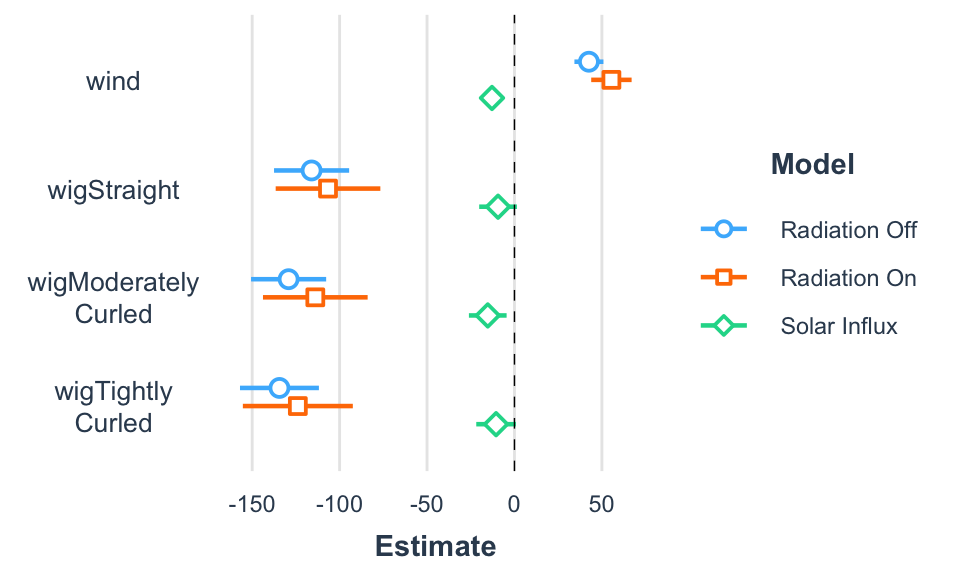
\includegraphics[width=0.6\linewidth]{/Users/tinalasisi-usc/GitHub/HairManikin2023/output/pdf/analysis_files/figure-latex/plt-summary-models-wet-1} 

}

\caption{Regression coefficients across regression models.}\label{fig:plt-summary-models-wet}
\end{figure}

\hypertarget{evaporative-heat-anova-plots}{%
\subsubsection{Evaporative heat ANOVA
plots}\label{evaporative-heat-anova-plots}}

\begin{figure}

{\centering 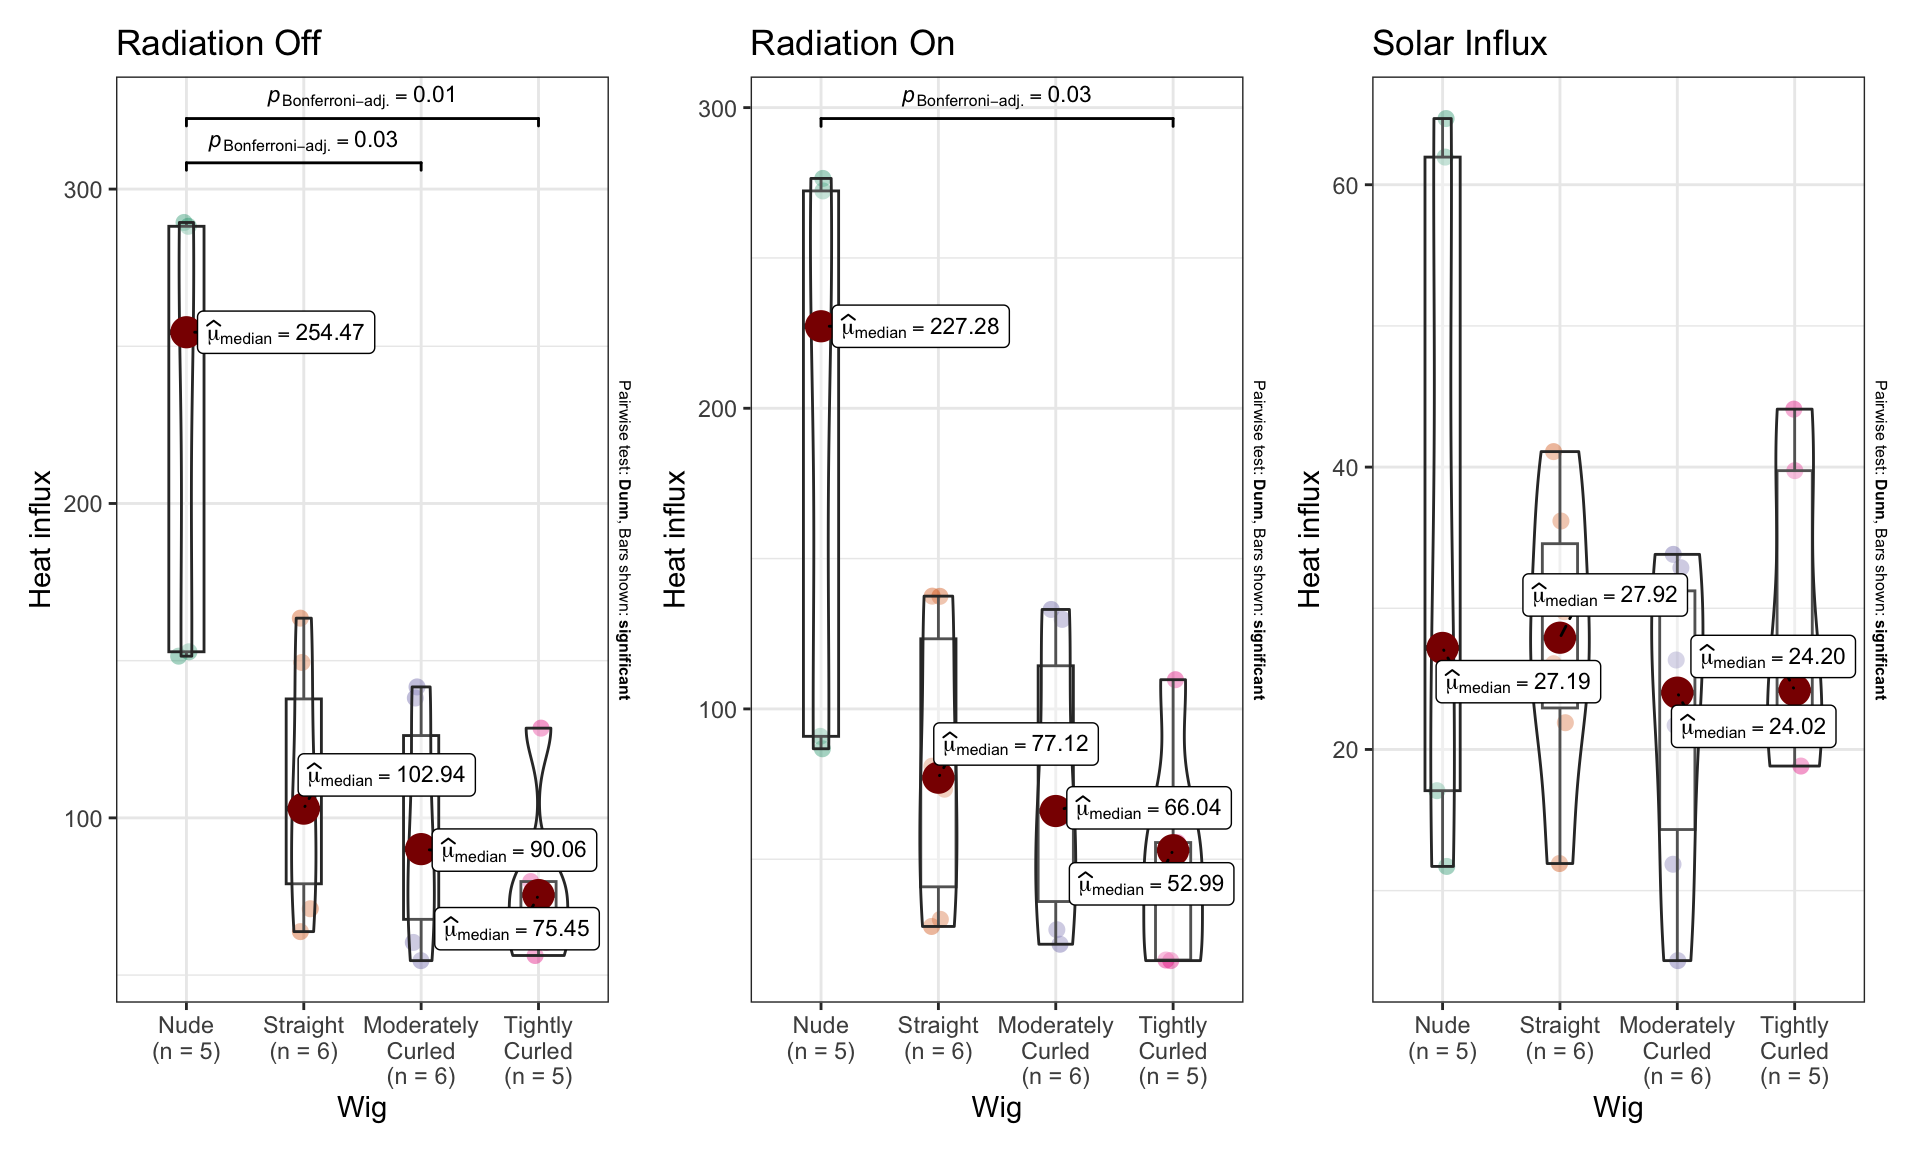
\includegraphics[width=0.95\linewidth]{/Users/tinalasisi-usc/GitHub/HairManikin2023/output/pdf/analysis_files/figure-latex/ggbetweenstats-wet-1} 

}

\caption{ANOVA of evaporative heat loss}\label{fig:ggbetweenstats-wet}
\end{figure}

\hypertarget{calculating-thermal-resistance}{%
\section{Calculating Thermal
Resistance}\label{calculating-thermal-resistance}}

\[I_t = \frac{T_{Skin} - T_{Air}}{H_{Dry}}\]

\begin{Shaded}
\begin{Highlighting}[]
\NormalTok{df\_wetdry[}\StringTok{"dry\_heat\_resistance"}\NormalTok{] }\OtherTok{\textless{}{-}}\NormalTok{ (df\_wetdry[}\StringTok{"skin\_temp"}\NormalTok{] }\SpecialCharTok{{-}}
\NormalTok{    df\_wetdry[}\StringTok{"amb\_temp"}\NormalTok{])}\SpecialCharTok{/}\NormalTok{df\_wetdry[}\StringTok{"heat\_loss"}\NormalTok{]}

\CommentTok{\# For the dry data, leave this blank}
\NormalTok{df\_wetdry }\OtherTok{\textless{}{-}}\NormalTok{ df\_wetdry }\SpecialCharTok{\%\textgreater{}\%}
    \FunctionTok{mutate}\NormalTok{(}\AttributeTok{dry\_heat\_resistance =} \FunctionTok{ifelse}\NormalTok{(wet\_dry }\SpecialCharTok{==} \StringTok{"wet"}\NormalTok{,}
        \ConstantTok{NaN}\NormalTok{, dry\_heat\_resistance))}
\end{Highlighting}
\end{Shaded}

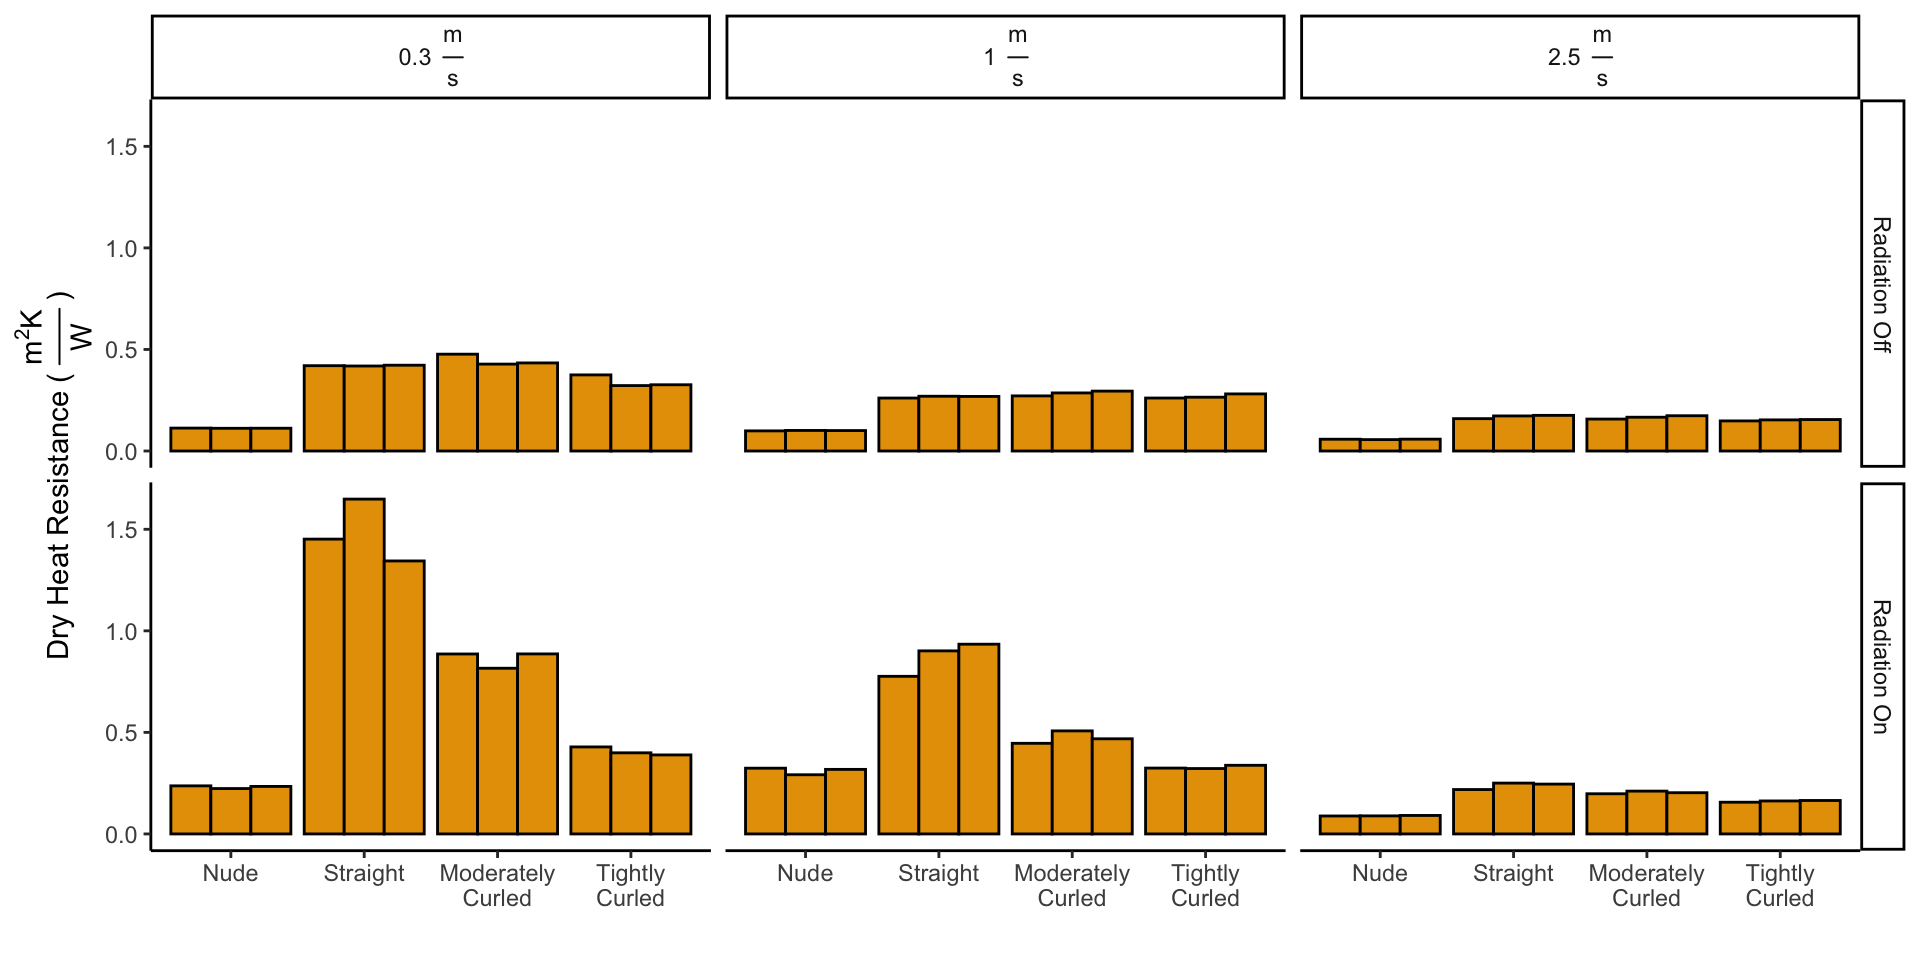
\includegraphics[width=0.95\linewidth]{/Users/tinalasisi-usc/GitHub/HairManikin2023/output/pdf/analysis_files/figure-latex/Thermal-Resistance-Plots-1}

\hypertarget{calculating-net-solar-influx}{%
\section{Calculating Net Solar
Influx}\label{calculating-net-solar-influx}}

\[I_{Dry} = H_{Dry} - H_{Dry}^{Solar}\]
\[I_{Evap} = H_{Evap} - H_{Evap}^{Solar}\]

\begin{Shaded}
\begin{Highlighting}[]
\CommentTok{\# Average all trials with the same characteristics}
\NormalTok{df\_averaged\_trials }\OtherTok{\textless{}{-}}\NormalTok{ df\_wetdry }\SpecialCharTok{\%\textgreater{}\%}
    \FunctionTok{group\_by}\NormalTok{(wig, wind, radiation, wet\_dry) }\SpecialCharTok{\%\textgreater{}\%}
    \FunctionTok{drop\_na}\NormalTok{(heat\_loss) }\SpecialCharTok{\%\textgreater{}\%}
    \FunctionTok{summarise}\NormalTok{(}\AttributeTok{heat\_loss =} \FunctionTok{mean}\NormalTok{(heat\_loss))}

\CommentTok{\# Pivot the dataframe to incldue radiation on and off}
\CommentTok{\# as part of same event}
\NormalTok{df\_radiation\_split }\OtherTok{\textless{}{-}}\NormalTok{ df\_averaged\_trials }\SpecialCharTok{\%\textgreater{}\%}
    \FunctionTok{pivot\_wider}\NormalTok{(}\AttributeTok{names\_from =} \FunctionTok{c}\NormalTok{(radiation), }\AttributeTok{values\_from =} \FunctionTok{c}\NormalTok{(heat\_loss)) }\SpecialCharTok{\%\textgreater{}\%}
    \FunctionTok{rename}\NormalTok{(}\AttributeTok{heat\_loss\_off =}\NormalTok{ off) }\SpecialCharTok{\%\textgreater{}\%}
    \FunctionTok{rename}\NormalTok{(}\AttributeTok{heat\_loss\_on =}\NormalTok{ on)}

\CommentTok{\# Calculate the net influx}
\NormalTok{df\_net\_influx\_plots }\OtherTok{\textless{}{-}}\NormalTok{ df\_radiation\_split }\SpecialCharTok{\%\textgreater{}\%}
    \FunctionTok{group\_by}\NormalTok{(wig, wind) }\SpecialCharTok{\%\textgreater{}\%}
    \FunctionTok{summarise}\NormalTok{(}\AttributeTok{wet\_dry =}\NormalTok{ wet\_dry, }\AttributeTok{net\_influx =}\NormalTok{ heat\_loss\_off }\SpecialCharTok{{-}}
\NormalTok{        heat\_loss\_on)}

\NormalTok{df\_net\_influx }\OtherTok{\textless{}{-}}\NormalTok{ df\_net\_influx\_plots }\SpecialCharTok{\%\textgreater{}\%}
    \FunctionTok{spread}\NormalTok{(wet\_dry, net\_influx)}
\end{Highlighting}
\end{Shaded}

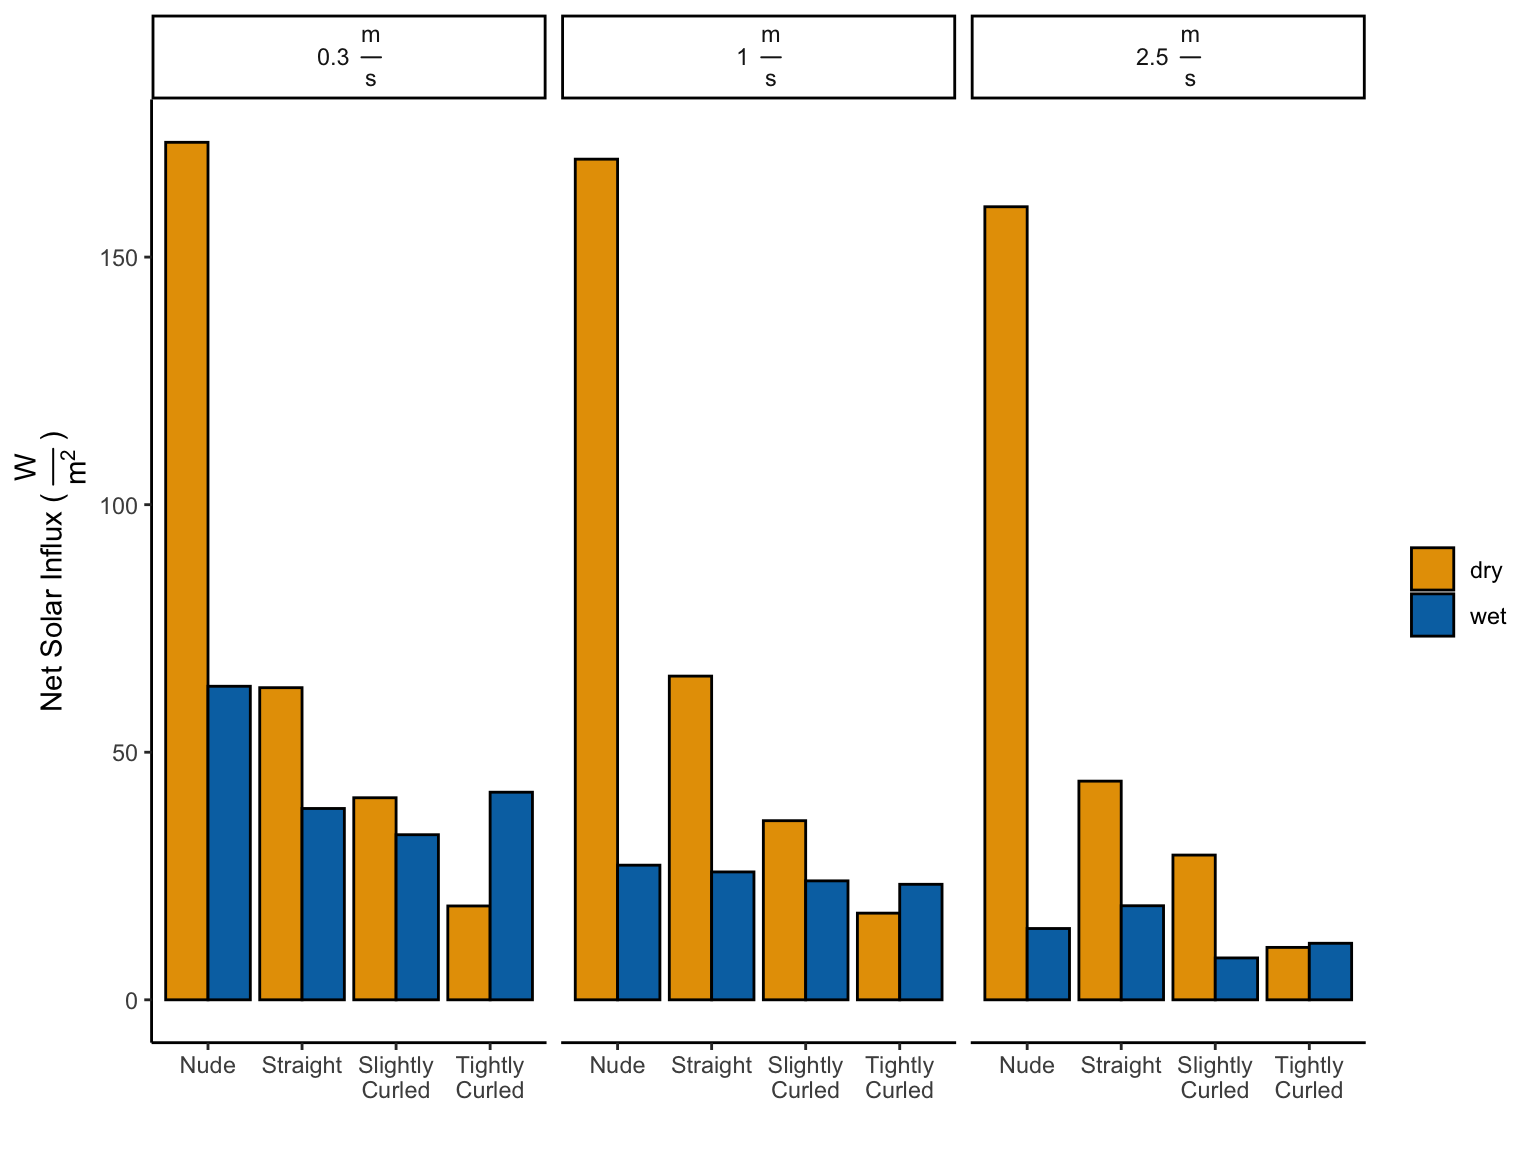
\includegraphics[width=0.95\linewidth]{/Users/tinalasisi-usc/GitHub/HairManikin2023/output/pdf/analysis_files/figure-latex/net-solar-influx-plts-1}
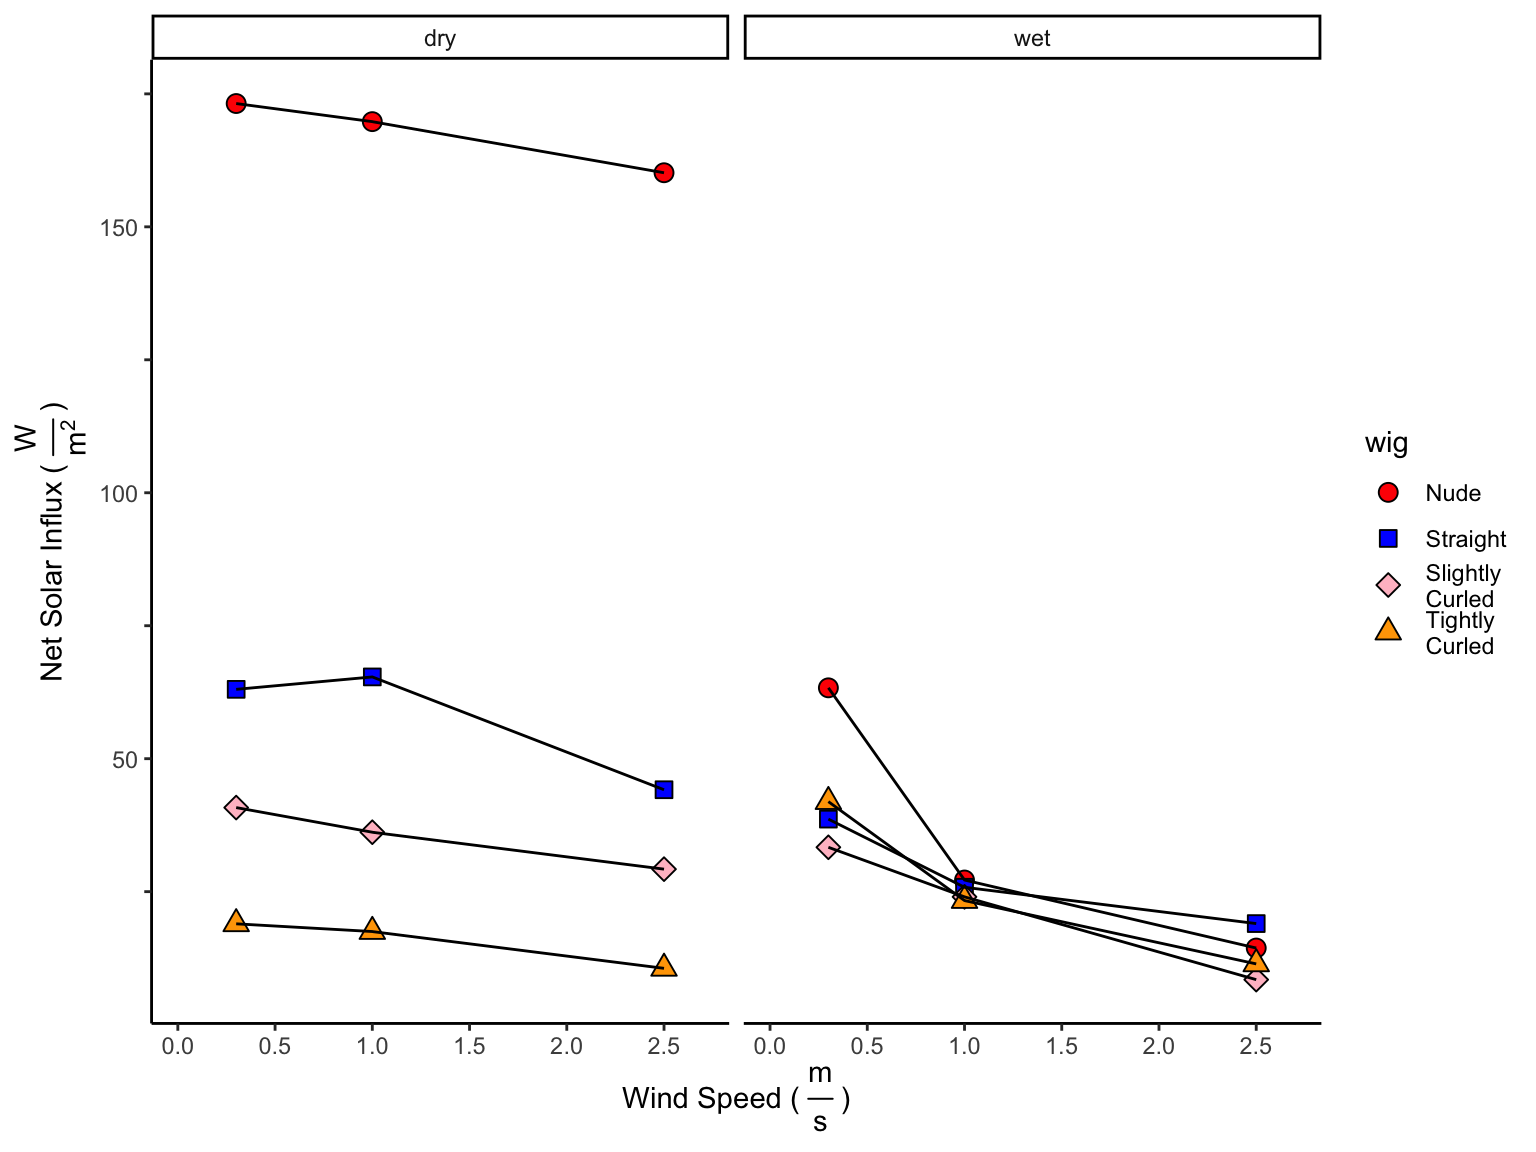
\includegraphics[width=0.95\linewidth]{/Users/tinalasisi-usc/GitHub/HairManikin2023/output/pdf/analysis_files/figure-latex/net-solar-influx-plts-2}

\hypertarget{adjusting-heat-losses-to-30-degrees-celsius}{%
\section{Adjusting Heat Losses to 30 Degrees
Celsius}\label{adjusting-heat-losses-to-30-degrees-celsius}}

\hypertarget{dry-heat-loss}{%
\subsection{Dry Heat Loss}\label{dry-heat-loss}}

\[H_{Dry}^{30^\circ C} = \frac{35 -30}{I_t}\]

\begin{Shaded}
\begin{Highlighting}[]
\CommentTok{\# Their calculation}
\NormalTok{df\_wetdry[}\StringTok{"heat\_30"}\NormalTok{] }\OtherTok{=}\NormalTok{ (}\DecValTok{35} \SpecialCharTok{{-}} \DecValTok{30}\NormalTok{)}\SpecialCharTok{/}\NormalTok{df\_wetdry[}\StringTok{"dry\_heat\_resistance"}\NormalTok{]}

\CommentTok{\# What I would expect df\_wetdry[\textquotesingle{}heat\_30\textquotesingle{}] =}
\CommentTok{\# (df\_wetdry[\textquotesingle{}skin\_temp\textquotesingle{}] {-} 30) /}
\CommentTok{\# df\_wetdry[\textquotesingle{}dry\_heat\_resistance\textquotesingle{}]}


\CommentTok{\# Recreate the radiation split dataframe to include}
\CommentTok{\# heat\_30}
\NormalTok{df\_averaged\_trials }\OtherTok{\textless{}{-}}\NormalTok{ df\_wetdry }\SpecialCharTok{\%\textgreater{}\%}
    \FunctionTok{group\_by}\NormalTok{(wig, wind, radiation, wet\_dry) }\SpecialCharTok{\%\textgreater{}\%}
    \FunctionTok{drop\_na}\NormalTok{(heat\_loss) }\SpecialCharTok{\%\textgreater{}\%}
    \FunctionTok{summarise}\NormalTok{(}\AttributeTok{heat\_loss =} \FunctionTok{mean}\NormalTok{(heat\_loss), }\AttributeTok{heat\_30 =} \FunctionTok{mean}\NormalTok{(heat\_30))}

\NormalTok{df\_radiation\_split }\OtherTok{\textless{}{-}}\NormalTok{ df\_averaged\_trials }\SpecialCharTok{\%\textgreater{}\%}
    \FunctionTok{pivot\_wider}\NormalTok{(}\AttributeTok{names\_from =} \FunctionTok{c}\NormalTok{(radiation), }\AttributeTok{values\_from =} \FunctionTok{c}\NormalTok{(heat\_loss,}
\NormalTok{        heat\_30))}
\end{Highlighting}
\end{Shaded}

\hypertarget{dry-and-wet-heat-losses-with-solar-radiation}{%
\subsection{Dry and Wet Heat Losses With Solar
Radiation}\label{dry-and-wet-heat-losses-with-solar-radiation}}

\[H_{Dry}^{30^{\circ} C,\:Solar} = H_{Dry}^{30^{\circ} C} - I_{Dry}\]
\[H_{Wet}^{30^{\circ} C,\:Solar} = H_{Evap + Dry}^{30^{\circ} C} = H_{Evap} + I_{Dry} + H_{Dry}^{30^{\circ} C,\:Solar}\]

\begin{Shaded}
\begin{Highlighting}[]
\NormalTok{dry\_heat\_30 }\OtherTok{=}\NormalTok{ df\_radiation\_split[df\_radiation\_split}\SpecialCharTok{$}\NormalTok{wet\_dry }\SpecialCharTok{==}
    \StringTok{"dry"}\NormalTok{, ]}

\NormalTok{heat\_evap }\OtherTok{=}\NormalTok{ df\_radiation\_split[df\_radiation\_split}\SpecialCharTok{$}\NormalTok{wet\_dry }\SpecialCharTok{==}
    \StringTok{"wet"}\NormalTok{, ]}


\NormalTok{df\_adjusted\_solar }\OtherTok{\textless{}{-}} \FunctionTok{data.frame}\NormalTok{(dry\_heat\_loss }\OtherTok{\textless{}{-}}\NormalTok{ dry\_heat\_30}\SpecialCharTok{$}\NormalTok{heat\_30\_off }\SpecialCharTok{{-}}
\NormalTok{    df\_net\_influx}\SpecialCharTok{$}\NormalTok{dry, wind }\OtherTok{\textless{}{-}}\NormalTok{ dry\_heat\_30}\SpecialCharTok{$}\NormalTok{wind, wig }\OtherTok{\textless{}{-}}\NormalTok{ dry\_heat\_30}\SpecialCharTok{$}\NormalTok{wig) }\SpecialCharTok{\%\textgreater{}\%}
    \FunctionTok{rename}\NormalTok{(}\AttributeTok{dry\_heat\_loss =} \StringTok{"dry\_heat\_loss....dry\_heat\_30.heat\_30\_off...df\_net\_influx.dry"}\NormalTok{) }\SpecialCharTok{\%\textgreater{}\%}
    \FunctionTok{rename}\NormalTok{(}\AttributeTok{wind =} \StringTok{"wind....dry\_heat\_30.wind"}\NormalTok{) }\SpecialCharTok{\%\textgreater{}\%}
    \FunctionTok{rename}\NormalTok{(}\AttributeTok{wig =} \StringTok{"wig....dry\_heat\_30.wig"}\NormalTok{)}


\NormalTok{df\_adjusted\_solar[}\StringTok{"wet\_heat\_loss"}\NormalTok{] }\OtherTok{\textless{}{-}} \SpecialCharTok{+}\NormalTok{heat\_evap}\SpecialCharTok{$}\NormalTok{heat\_loss\_on }\SpecialCharTok{+}
\NormalTok{    df\_net\_influx}\SpecialCharTok{$}\NormalTok{dry }\SpecialCharTok{+}\NormalTok{ df\_adjusted\_solar}\SpecialCharTok{$}\NormalTok{dry\_heat\_loss}


\NormalTok{df\_adjusted\_solar\_plots }\OtherTok{\textless{}{-}}\NormalTok{ df\_adjusted\_solar }\SpecialCharTok{\%\textgreater{}\%}
    \FunctionTok{pivot\_longer}\NormalTok{(}\AttributeTok{cols =} \FunctionTok{c}\NormalTok{(}\StringTok{"dry\_heat\_loss"}\NormalTok{, }\StringTok{"wet\_heat\_loss"}\NormalTok{),}
        \AttributeTok{names\_to =} \StringTok{"wet\_dry"}\NormalTok{, }\AttributeTok{values\_to =} \StringTok{"heat\_loss"}\NormalTok{)}
\end{Highlighting}
\end{Shaded}

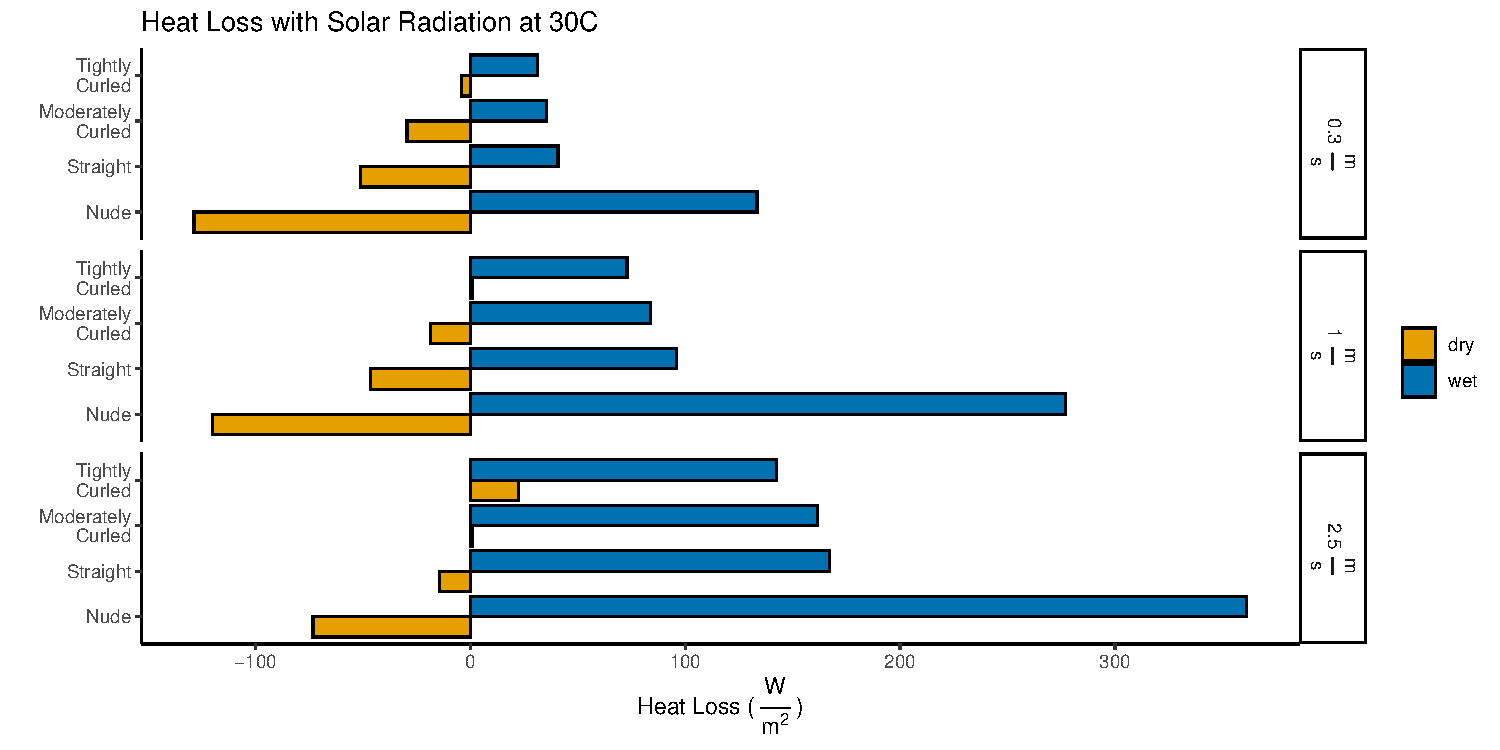
\includegraphics[width=0.95\linewidth]{/Users/tinalasisi-usc/GitHub/HairManikin2023/output/pdf/analysis_files/figure-latex/plt-heatloss-radiation-1}
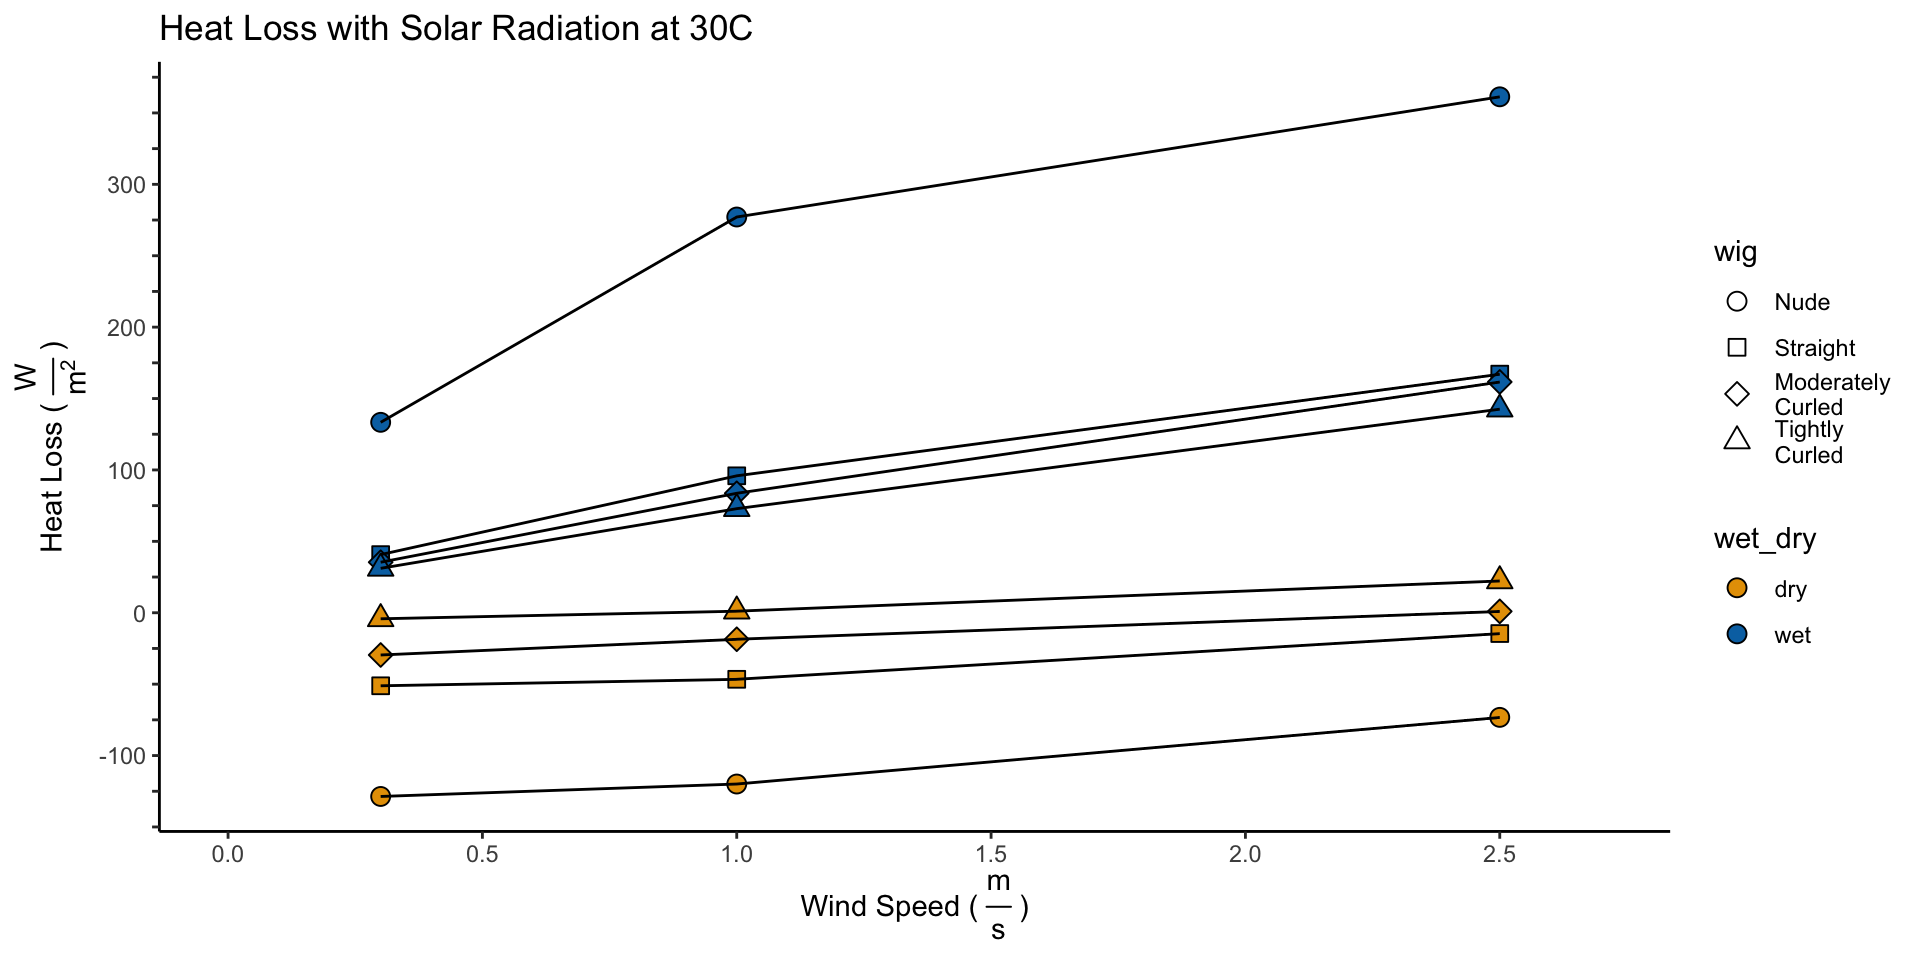
\includegraphics[width=0.95\linewidth]{/Users/tinalasisi-usc/GitHub/HairManikin2023/output/pdf/analysis_files/figure-latex/plt-heatloss-radiation-2}

\hypertarget{calculating-evaporative-potential}{%
\section{Calculating Evaporative
Potential}\label{calculating-evaporative-potential}}

\[H_{Max}^{30^{\circ} C,\:Solar} = H_{Wet}^{30^{\circ} C,\:Solar} - H_{Dry}^{30^{\circ} C,\:Solar}\]

\begin{Shaded}
\begin{Highlighting}[]
\NormalTok{df\_evaporative\_potential }\OtherTok{\textless{}{-}}\NormalTok{ df\_adjusted\_solar}\SpecialCharTok{$}\NormalTok{wet\_heat\_loss }\SpecialCharTok{{-}}
\NormalTok{    df\_adjusted\_solar}\SpecialCharTok{$}\NormalTok{dry\_heat\_loss}
\end{Highlighting}
\end{Shaded}

\hypertarget{calculating-sweat-requirements}{%
\section{Calculating Sweat
Requirements}\label{calculating-sweat-requirements}}

\[Sweat_{Max} = \frac{H_{Max}^{30^{\circ} C,\:Solar} * 3600}{2430}\]

\[ IF \; H_{Dry}^{30^{\circ} C,\:Solar} < 0, \; Sweat_{Zero} = -\frac{H_{Dry}^{30^{\circ} C,\:Solar} * 3600}{2430} \\
ELSE, \; Sweat_{Zero} = 0\]

\begin{Shaded}
\begin{Highlighting}[]
\CommentTok{\# Create a new df with the sweat requirements}

\NormalTok{df\_sweat\_requirements }\OtherTok{\textless{}{-}} \FunctionTok{data.frame}\NormalTok{(sweat\_max }\OtherTok{\textless{}{-}}\NormalTok{ df\_evaporative\_potential }\SpecialCharTok{*}
    \DecValTok{3600}\SpecialCharTok{/}\DecValTok{2430}\NormalTok{, sweat\_zero }\OtherTok{\textless{}{-}} \SpecialCharTok{{-}}\DecValTok{3600}\SpecialCharTok{/}\DecValTok{2430} \SpecialCharTok{*}\NormalTok{ df\_adjusted\_solar[}\StringTok{"dry\_heat\_loss"}\NormalTok{],}
\NormalTok{    wig }\OtherTok{\textless{}{-}}\NormalTok{ df\_adjusted\_solar}\SpecialCharTok{$}\NormalTok{wig, wind }\OtherTok{\textless{}{-}}\NormalTok{ df\_adjusted\_solar}\SpecialCharTok{$}\NormalTok{wind)}

\CommentTok{\# Rename columns}
\FunctionTok{colnames}\NormalTok{(df\_sweat\_requirements) }\OtherTok{\textless{}{-}} \FunctionTok{c}\NormalTok{(}\StringTok{"sweat\_max"}\NormalTok{, }\StringTok{"sweat\_zero"}\NormalTok{,}
    \StringTok{"wig"}\NormalTok{, }\StringTok{"wind"}\NormalTok{)}


\CommentTok{\# Replace all values less than 0 with 0 per formula}
\NormalTok{df\_sweat\_requirements[}\StringTok{"sweat\_zero"}\NormalTok{][df\_sweat\_requirements[}\StringTok{"sweat\_zero"}\NormalTok{] }\SpecialCharTok{\textless{}}
    \DecValTok{0}\NormalTok{] }\OtherTok{\textless{}{-}} \DecValTok{0}
\end{Highlighting}
\end{Shaded}

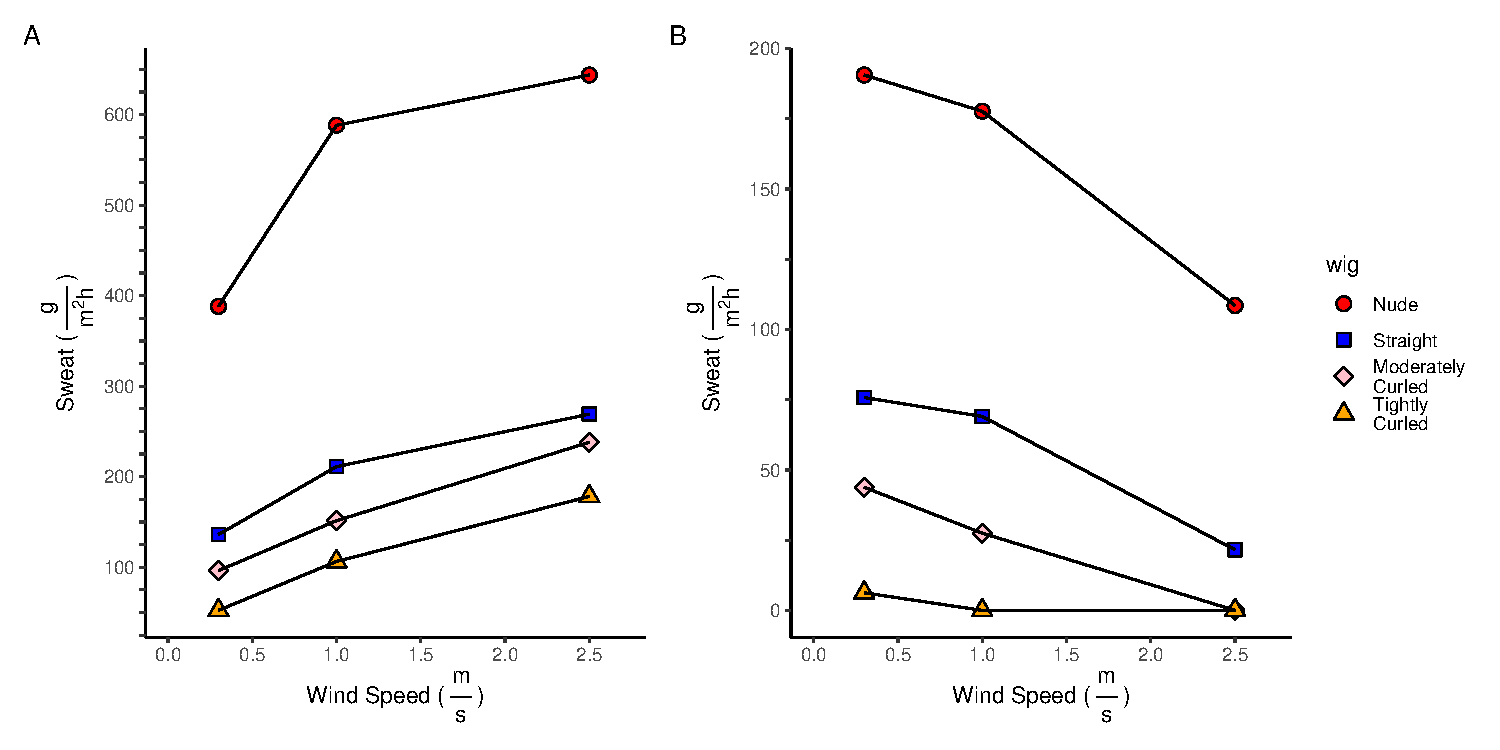
\includegraphics[width=0.95\linewidth]{/Users/tinalasisi-usc/GitHub/HairManikin2023/output/pdf/analysis_files/figure-latex/plt-sweat-req-1}

\end{document}
